\documentclass[a4paper,11pt,twoside,openright]{book}

\usepackage[spanish]{babel}
\usepackage[utf8]{inputenc}

\usepackage{eurosym}
\usepackage{fancybox}
\usepackage{multicol}
\usepackage{amsmath}
\usepackage{subcaption}
\usepackage[nottoc,numbib]{tocbibind}
\usepackage[pdftex,usenames,dvipsnames]{color}
\usepackage{float}
% compilar con pdflatex.
\usepackage[pdftex]{graphicx}


\usepackage{setspace}
\onehalfspacing
\usepackage{geometry}
\geometry{
  inner=3.5cm,
  outer=2.5cm,
  bottom=3.5cm,
  top=3.5cm}

\usepackage{fancyhdr}
\pagestyle{fancy}
\fancyhf{}
\fancyhf[HR]{\thepage}
\fancyhf[HL]{\nouppercase\rightmark}

\usepackage{booktabs}
\usepackage{hyperref}
\hypersetup{
    colorlinks,
    linkcolor={red!50!black},
    citecolor={blue!50!black},
    urlcolor={blue!80!black}
}
\usepackage{rotating}
\usepackage{multicol}
\usepackage{multirow}
\usepackage{pgfgantt}
\usepackage{enumitem}
\usepackage{color}
\usepackage{xcolor}
\usepackage{caption}
\DeclareCaptionFont{white}{\color{white}}
\DeclareCaptionFormat{listing}{\colorbox{gray}{\parbox{\textwidth}{#1#2#3}}}
\captionsetup[lstlisting]{format=listing,labelfont=white,textfont=white}

 \usepackage{listings}
 \usepackage{courier}
 \lstset{
         basicstyle=\footnotesize\ttfamily, % Standardschrift
         numberstyle=\tiny,          % Stil der Zeilennummern
         numbersep=5pt,              % Abstand der Nummern zum Text
         tabsize=2,                  % Groesse von Tabs
         extendedchars=true,         %
         breaklines=true,            % Zeilen werden Umgebrochen
         keywordstyle=\textbf,
         frame=b,
         stringstyle=\textit, % Farbe der String
         showspaces=false,           % Leerzeichen anzeigen ?
         showtabs=false,             % Tabs anzeigen ?
         xleftmargin=17pt,
         framexleftmargin=17pt,
         framexrightmargin=5pt,
         framexbottommargin=4pt,
         %backgroundcolor=\color{lightgray},
         showstringspaces=false      % Leerzeichen in Strings anzeigen ?
 }

 \lstset{literate=
  {á}{{\'a}}1 {é}{{\'e}}1 {í}{{\'i}}1 {ó}{{\'o}}1 {ú}{{\'u}}1
  {Á}{{\'A}}1 {É}{{\'E}}1 {Í}{{\'I}}1 {Ó}{{\'O}}1 {Ú}{{\'U}}1
  {à}{{\`a}}1 {è}{{\`e}}1 {ì}{{\`i}}1 {ò}{{\`o}}1 {ù}{{\`u}}1
  {À}{{\`A}}1 {È}{{\'E}}1 {Ì}{{\`I}}1 {Ò}{{\`O}}1 {Ù}{{\`U}}1
  {ä}{{\"a}}1 {ë}{{\"e}}1 {ï}{{\"i}}1 {ö}{{\"o}}1 {ü}{{\"u}}1
  {Ä}{{\"A}}1 {Ë}{{\"E}}1 {Ï}{{\"I}}1 {Ö}{{\"O}}1 {Ü}{{\"U}}1
  {â}{{\^a}}1 {ê}{{\^e}}1 {î}{{\^i}}1 {ô}{{\^o}}1 {û}{{\^u}}1
  {Â}{{\^A}}1 {Ê}{{\^E}}1 {Î}{{\^I}}1 {Ô}{{\^O}}1 {Û}{{\^U}}1
  {œ}{{\oe}}1 {Œ}{{\OE}}1 {æ}{{\ae}}1 {Æ}{{\AE}}1 {ß}{{\ss}}1
  {ç}{{\c c}}1 {Ç}{{\c C}}1 {ø}{{\o}}1 {å}{{\r a}}1 {Å}{{\r A}}1
  {€}{{\EUR}}1 {£}{{\pounds}}1
 }

\parskip=6pt

\parindent=10pt

\setcounter{secnumdepth}{3}

\title{Desarrollo de un videojuego roguelike para invidentes aplicando técnicas de Procesamiento del Lenguaje Natural.}
\author{Darío Penas Sabín}
\date{\today}


\renewcommand\lstlistingname{Fragmento de Código}
\renewcommand\lstlistlistingname{Fragmentos de Código}

\newenvironment{bottompar}{\par\vspace*{\fill}}{\clearpage}

\begin{document}
        %
% Portada.
%

% Nota: Sería más cómodo emplear el comando \maketitle que genera una portada de forma automática, pero
% no incluye toda la información que es necesario incluir en la memoria de un proyecto de fin de carrera
% de la Facultad de Informática de A Coruña.
%

\begin{titlepage}

	\begin{center}

		% Logotipo de la universidad.
		
\includegraphics[width=6cm]{./eps/logo_udc.eps}
		\vspace{2cm}

		{\Large{\textbf{Facultade de Informática da Universidade de A Coruña}}}
		\\
		{\it \large{\textbf{Computación}}}
		\vspace{1cm}

		% Indicamos el nombre de la titulación oficial que hemos cursado con tanto esfuerzo.
		{\large PROYECTO DE FIN DE CARRERA\\Ingeniería Informática}
		\vspace{1cm}

		% Título
		\textbf{\Large Desarrollo de un videojuego roguelike para invidentes aplicando técnicas de Procesamiento del Lenguaje Natural.}
		\vspace{7cm}
	\end{center}

	\begin{flushright}
		\begin{tabular}{ll}
			\large{\textbf{Alumno:}}	&
			\large{Darío Penas Sabín} \\

			% Nombre del director/tutor del proyecto.
			\large{\textbf{Director:}}	&
			\large{Jesús Vilares Ferro} \\

			% Nombre del director/tutor del proyecto.
			\large{\textbf{Director:}}	&
			\large{Carlos Gómez Rodríguez} \\

			% Fecha.
			\large{\textbf{Fecha:}}	&
			\large{CHANGE: 15 de junio de 2016} \\
		\end{tabular}
	\end{flushright}

\end{titlepage}


        \frontmatter

        \thispagestyle{empty}

        \section*{Resumen:}

La industria del entretenimiento digital ha crecido inmensamente en los últimos años, llegando a alcanzar números de ventas jamás vistos anteriormente.
Parte de la razón de este crecimiento viene dada por una mejora radical en el aspecto visual, necesaria para que el jugador se sienta inmerso en la aventura que se le está planteando.
Estas mejoras, sin embargo, dejan de lado a muchos jugadores que, por diferentes motivos, no son capaces de apreciar el contenido visual que se les ofrece o tienen problemas para ello, haciendo imposible que disfruten del contenido ofrecido.

Este proyecto consiste en la creación de un videojuego de género \textit{roguelike} para invidentes que, desde un principio, parte de la idea de generar contenido específicamente diseñado para que pueda ser jugado por todo el mundo, haciendo énfasis en ofrecer al jugador una diversa cantidad de frases que describan lo que está sucediendo en su alrededor y que serán generadas automáticamente en base a una serie de gramáticas y diccionarios, empleando para ello técnicas de Procesamiento del Lenguaje Natural.

        \thispagestyle{empty}

        \section*{Lista de palabras clave:}

\begin{itemize}
  \item Tiflotecnología
  \item Procesamiento del Lenguaje Natural
  \item Accesibilidad
  \item Entretenimiento Digital
  \item \textit{Roguelike}
  \item Java
  \item \textit{Open Source}
\end{itemize}

        \thispagestyle{empty}

        %
% Agradecimientos
%

\section*{Agradecimientos}

Me gustaría aprovechar este pequeño espacio para agredecer a todas las personas que me ayudaron, en diferentes niveles y formas, a elaborar y terminar este proyecto.

Gracias a todos aquellos que dedicaron parte de su tiempo a resolverme dudas sobre tiflotecnología y accesibilidad (sobre todo a los usuarios de \textit{Reddit} \textit{ais523} y \textit{fastfinge}), así como a todos los profesores que tuve durante los cinco años de carrera y que lograron que llegue al punto en el que me encuentro profesionalmente. En especial me gustaría agredecer a mis directores, Jesús y Carlos, el esfuerzo extra que han hecho durante este tiempo en el que he estado trabajando en el extranjero para mantenerme al tanto y resolverme dudas a distancia cuando estaba perdido.

Tampoco puedo olvidarme de todos los amigos que he hecho durante todos estos años y con los que he pasado tantas horas delante y fuera de la pantalla. Adrián (insaciable compañero de prácticas que me tuvo que aguantar durante tantos años), Daniel, Vanesa, Santi, Chava, Mónica, Brais, María, Xacobe y otros muchos. ¡Gracias por vuestra ayuda y amistad!

Por último, gracias a todas aquellas personas (especialmente a mis padres y a mi novia Diantha) que me ayudaron y presionaron a que terminara el proyecto cuanto antes y no lo dejara pasar.

¡Gracias a todos por todos estos maravillosos años!

\begin{flushright}
  Darío Penas Sabín \\
  Amsterdam, \today
\end{flushright}


        \thispagestyle{empty}

        \tableofcontents
        \listoffigures

        \mainmatter
        \chapter[Introdución]{Introdución}

En este capítulo introductorio se explicarán los aspectos necesarios para entender lo más importante del proyecto, la motivación para realización del mismo y un breve resumen del resto de capítulos que forman parte de la memoria.

\section{Videojuegos y personas invidentes}
La mayor parte de los videojuegos comerciales no tienen en cuenta a muchas minorías de la sociedad. Haciendo una pequeña búsqueda online pueden encontrarse miles de personas quejándose de \textit{first person shooters} que tienen un \textit{FOV}\footnote{\textit{Field of view}, campo de visión. Extensión de mundo observable en un momento dado} limitado, causándoles mareos al poco rato; daltónicos protestando que diferentes juegos (como por ejemplo The Witness\footnote{Juego de puzzles en primera persona: \url{http://the-witness.net/}}), basan buena parte de su mecánica en que el jugador sea capaz de distinguir diferentes colores; zurdos que tienen que acomodarse a ciertos controles a no existir una opción para cambiarlos; invidentes que no pueden disfrutar de prácticamente ninguno de los títulos que se encuentran en el mercado, etc.

En este proyecto nuestro objetivo es crear un videojuego desde cero que tenga en cuenta todo tipo de minorías, tomando especial relevancia el desarrollo para invidentes y centrándose en los aspectos que sean relevantes para ellos; descripciones que sean fácilmente reproducibles que cambien automáticamente y fácil expansión del título, tanto en características generales como en idiomas, gramáticas o palabras empleadas en el mismo.

\subsection{Visita a la \textit{ONCE}}
A principios de 2015 Jesús y yo fuimos a un taller de la ONCE donde una persona invidente nos habló sobre la tiflotecnología, nos mostró la forma en la que usaban ordenadores y móviles, incluso para leer código y los errores, muchos de ellos fácilmente solventables, que se cometían día a día en temas de accesibilidad. Esta visita nos abrió los ojos y gracias a ella fuimos capaces de detectar posibles mejoras que hacer al proyecto y los fallos que no deberíamos de cometer en su diseño. También se ofrecieron a probar el proyecto una vez estuviera listo, pero este será un tema que trataremos en las próximas secciones.

\section{Motivación}
El entretenimiento digital siempre ha sido parte de mi vida y una de las razones por las que desde pequeño estuve interesado en la informática y motivo por el que, finalmente, acabé estudiando esta carrera. Del mismo modo, y habiéndome relacionado con bastante gente con toda clase de necesidades especiales durante un gran periodo de tiempo, mi interés por la tiflotecnología y las limitaciones que la tecnología ofrece a millones de personas no hizo más que crecer año a año.

A pesar de los grandes avances de la industria de los videojuegos y de la gran cantidad de nuevos estudios y proyectos que se lanzan anualmente, resulta muy complicado poder dedicarse profesionalmente a cualquiera de estas dos cosas (y no digamos ambas a la vez) por lo que en mi futuro profesional no he sido capaz, al menos de momento, de cumplir mi sueño de trabajar en lo que más me apasiona. Por este motivo, cuando Jesús me comentó que él y Carlos llevaban un tiempo con este proyecto disponible, no dudé en un instante en aceptarlo y ponerme manos a la obra.

Este videojuego se ha desarrollado durante el periodo de un par de años en los que se incluyen muchos cambios en mi vida, tales como mi estancia permanente en Holanda hace ya casi dos años y mis primeros pasos en el mundo laboral. Cada día que pasa me alegro más de tener un proyecto como éste, dado que sin la pasión e interés por el mismo estoy seguro de que jamás lo habría terminado.

\section{Estructura de la memoria}

La memoria está formada por ocho capítulos en los que se explican los pasos tomados a la hora de crear el proyecto.

\paragraph*{Capítulo 1. Introducción.}
Se explicarán, de manera general y resumida, en qué consiste el proyecto, la motivación del mismo y la estructura que tendrá la memoria.

\paragraph*{Capítulo 2. Estado del arte.}
En este apartado hablaremos de otros proyectos similares, de la situación actual de la industria sobre el problema que tratamos en este proyecto y del diferente software que es utilizado en relación con la tiflotecnología.

\paragraph*{Capítulo 3. Fundamentos Tecnológicos.}
Citaremos y hablaremos sobre las herramientas y bibliotecas empleadas durante la elaboración del proyecto.

\paragraph*{Capítulo 4. Metodología.}
Se detallarán las prácticas y metodologías de desarrollo empleadas para la realización del videojuego y la razón de su uso.

\paragraph*{Capítulo 5. Planificación y Seguimento.}
Detallaremos la planificación y seguimiento usados en cada una de las etapas del proyecto. 

\paragraph*{Capítulo 6. Análisis de requisitos.}
Se comentará el análisis de requisitos para este proyecto y se explicará en detalle cada uno de los mismos.

\paragraph*{Capítulo 7. Diseño e implementación.}
En este capítulo explicaremos los detalles del diseño y de la implementación de ciertas partes del programa que consideramos más relevantes.

\paragraph*{Capítulo 8. Recepción, conclusión y trabajo futuro.}
En este apartado mostraremos los comentarios obtenidos por la comunidad durante el desarrollo del juego, se relatarán las conclusiones obtenidas y se detallarán los posibles cambios, mejoras y extras que se podrán tener en cuenta en el futuro para su mejora.

        \chapter{Estado del Arte}

En este capítulo hablaremos, principalmente, de dos importantes aspectos. El primero es la situación de la industria del entretenimiento digital hoy en día, seguido de una definición sobre lo que es un \textit{roguelike}. El segundo son los elementos que dificultan y facilitan el uso de diferentes programas y \textit{software} a ciertos sectores de la sociedad como invidentes o daltónicos; cómo algunos programas intentan solventar estos problemas y las razones por las que hemos elegido introducir ciertos elementos en nuestro proyecto para diliar con los mismos.

\section{La industria del entretenimiento digital en la actualidad}

Desde sus primeros pasos hasta hoy en día, tal y como sucede con muchas de las novedades en el mundo del entretenimiento y la cultura, el sector del ocio digital ha sufrido cierto estigma por una gran parte de la población, siendo censurado y degragado en mayor o menor medida, no tan solo por cierta parte de la sociedad al considerarlo como algo enfocado para niños y sin mucho interés o relevancia cultural, pero también por muchos medios de comunicación y gobiernos. A pesar de que hoy en día este problema todavía está activo\footnote{Es común que cada año en Australia se censuren algunos juegos como \href{http://goo.gl/hFrQah}{Paranautical Activity} por razones que otras formas de entretenimiento y cultura como películas o libros no se ven tan afectados.}, la industria se ha expandido tanto (consolas, ordenadores, navegadores, Facebook, móvil...), que cada vez es más complicado encontrar a alguien que no haya jugado a algún videojuego en las últimas semanas, ya es un elemento que forma parte del día a día de mucha parte de la población y defenderlo como un elemento de gran importancia cultural es cada vez más sencillo.

\subsection{La industria, en números}
En todo el mundo, pero especialmente en EEUU, la industria de los videojuegos es uno de los sectores con más crecimiento \cite{website:gamesimprovingeconomy} llegando a generar, solamente en ventas digitales, alrededor de 61 billones de dólares en el año 2015 \cite{website:gamingsales}.

Este gran éxito se debe, en gran parte, a la irrupción de los juegos desarrollados para móviles, cuyo beneficio ha ido aumentando enormemente durante los últimos años. \footnote{\href{http://goo.gl/Lz9UAa}{La venta de videojuegos en Alemania crece año tras año, pero el mayor aumento de beneficio se está centrando en el mercado de los juegos para móvil}}. Sin embargo, esto no significa que el resto de plataformas no estén triunfando o se hayan quedado estancadas. Solamente Steam, la plataforma de distribución digital para PC por excelencia que ha sido desarrollada por Valve, ha generado alrededor de 3 billones y medio de dólares en el año 2015\cite{website:steamgamesmarket}.

También hemos visto nuevas consolas salir al mercado hace poco más de dos años: PlayStation 4 y Xbox One. La primera de ellas ha logrado vender, a principios del año 2016, alrededor de 36 millones de unidades\cite{website:ps4sales}, mientras que la consola de Microsoft llega a los 19.1 millones en el mismo periodo\cite{xboxonesales}, haciendo un total de más de 55 millones de unidades en total, la cual es una gran cifra en comparación con los años anteriores.

Con el mercado del PC resurgiendo, las consolas de sobremesa obteniendo grandes números de ventas, las portátiles resistiendo la lucha contra los móviles, el mercado de los videojuegos para móvil en esplendor y los cascos de realidad virtual llegando al mercado este año 2016 y obteniendo grandes números de preventas; todo parece indicar que la industria de ocio digital no hará más que crecer durante los próximos años.

\subsection{Conclusión}

Lo que comenzó hace varias décadas como un modo de entretenimiento sin ninguna pretensión, generalmente enfocado a un público infantil o adolescente y que miraba a otras industrias como la cinematográfica con recelo, tanto en números como en visibilidad, se ha convertido en todo lo que había deseado y más. Gracias a grandes títulos y a su expansión a toda clase de dispositivos, no se puede hablar de la industria del entretenimiento sin hablar de videojuegos y, en muchos casos, algunos de esos títulos han logrado ser nombrados como obras de arte en su género, pasando a la historia y siendo recordados a lo largo de los años.

\section{\textit{Roguelikes.}}
\label{sec:roguelikeinformacion}

\subsection{Qué es y orígenes}

En 1983, Michael Toy y Glenn Wichman crearon un videojuego llamado Rogue\footnote{Desde 2014 este juego se encuentra disponible en \href{https://archive.org/details/msdos_Rogue_1983}{archive.org}} que acabó definiendo un género que sigue vigente y en gran esplendor hoy en día.

Las características principales que definieron a Rogue y que, por extensión, definieron al género de los \textit{roguelikes} inicialmente son:

\paragraph{Dificultad}: Rogue es un videojuego difícil con \textit{permadeath}\footnote{Una vez que el jugador muere, tiene que empezar desde el principio; no hay partidas guardadas} que obligará al jugador a rejugarlo una y otra vez, intentando llegar más lejos que la anterior partida gracias a ir aprendiendo los funcionamientos del mismo.

\paragraph{Aleatoriedad}: Cada vez que el jugador comienza una partida nueva se encontrará con ciertos elementos que han cambiado con respecto a la vez anterior: el mapa es distinto, los elementos y enemigos se encuentran en sitios diferentes, los objetos obtenidos han cambiado... causando que cada vez que el usuario empiece, tenga un grado de dificultad pseudo-aleatorio dependiendo de la semilla con la que estos elementos hayan sido generados.

\paragraph{Progresión}: Una de las frases más escuchadas en las críticas positivas que Rogue recibió tras su lanzamiento es que el jugador sentía la necesidad de intentar llegar más lejos en cada una de las partidas jugadas\cite{website:machinesnetworks}. Esto viene dado, sobre todo, por la sensación de progresión y de que en cada \textit{run}\footnote{Palabra comúnmente usada en estos géneros y que se refiere a una partida desde su inicio hasta que el jugador pierde} el usuario vaya mejorando. Dentro de la propia partida también existe una progresión a medida que el usuario derrota enemigos, consiguiendo puntos de experiencia, subiendo niveles y obteniendo mejores armas y armaduras con las que ser un poco más fuerte. La intriga por saber los nuevos objetos que se pueden conseguir, así como los nuevos enemigos con los que nos enfrentaremos y mapas que se generarán, hace que \textit{Rogue} fuera fácilmente rejugable e interesante para todo tipo de usuarios.

\begin{figure}[h!]
		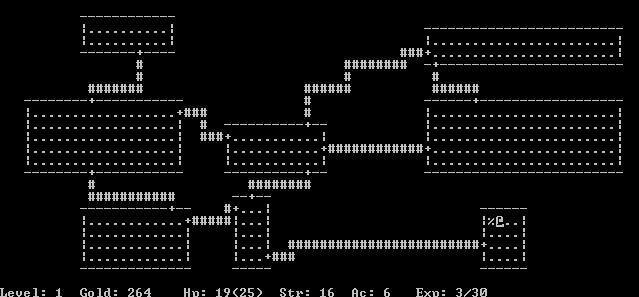
\includegraphics[width=\textwidth,height=\textheight,keepaspectratio]{./img/roguegame.PNG}
	\caption{Captura de pantalla de \href{https://en.wikipedia.org/wiki/File:Rogue_Unix_Screenshot_CAR.PNG}{dominio público} (tal y como todas las imágenes mostradas en este proyecto) del videojuego Rogue}
	\label{fig:roguegame}
\end{figure}

A partir de este momento muchos fueron los juegos que decidieron imitar estas características de Rogue, añadiendo, cambiando o enfatizando diferentes elementos. Por este motivo es por lo que se denominan \textit{roguelikes}, dado que siguen los pasos marcados por \textit{Rogue}0.

\subsection{En la actualidad}

Tras el éxito de Rogue, fueron muchos los títulos que simularon su fórmula de éxito e intentaron mejorarlo, sobre todo gráficamente. Algunos de ellos se centran en diferentes aspectos (combate en vez de exploración, por ejemplo) y llegan a ser completamente diferentes a la hora de jugarlos (por turnos o tiempo real) pero, sin embargo, todos conservan buena parte de las características que hicieron al género famoso hasta hoy en día.

\begin{figure}[h!]
		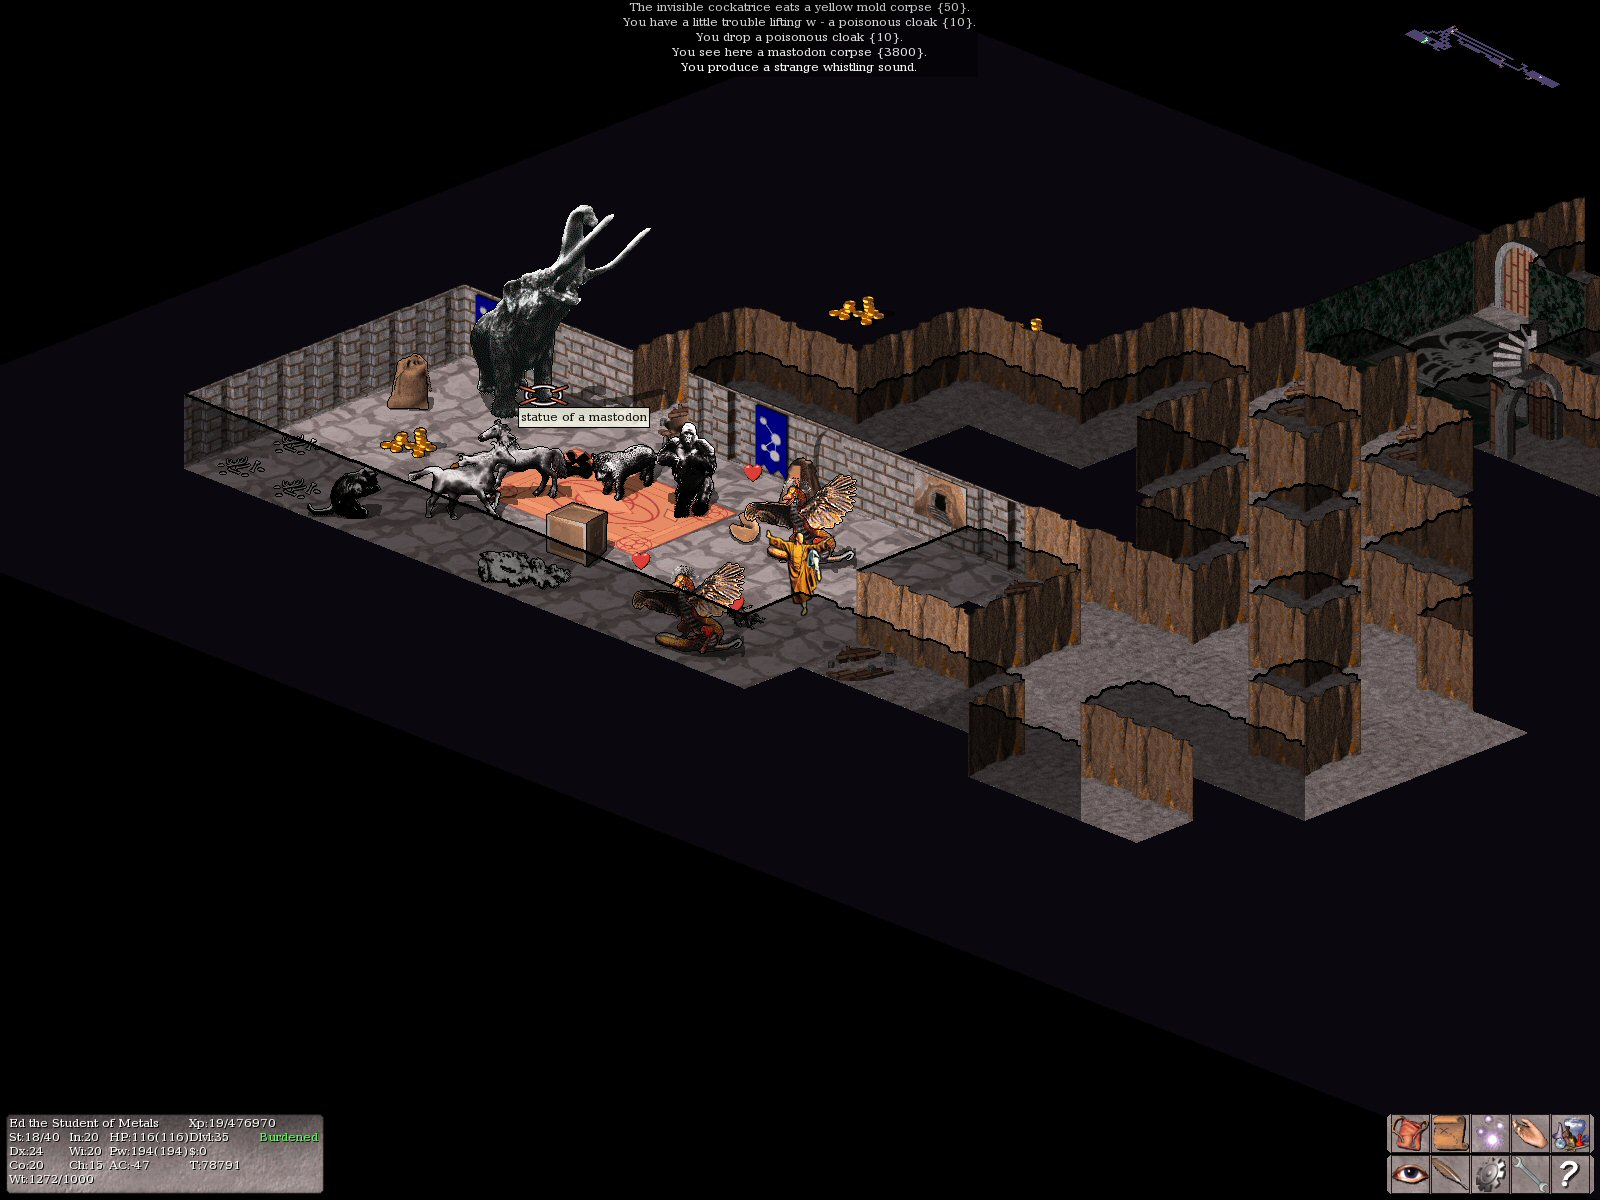
\includegraphics[width=\textwidth,height=\textheight,keepaspectratio]{./img/Vultures.jpg}
	\caption{Captura de pantalla del videojuego Vultures}
	\label{fig:vulturesgame}
\end{figure}

Incluso una gran cantidad de nuevos títulos, muchos de ellos desarrollados por empresas independientes, no dan especial importancia a tener gráficos en 3D o texturas increíbles, sino que optan por profundizar en crear una ambientación interesante y ofrecer un sistema de combate y exploración únicos y pulidos.
Uno de estos títulos que ha triunfado enormemente desde su lanzamiento en 2012 fue FTL. Hemos adjuntado una captura de pantalla \ref{fig:ftl} como referencia.

\begin{figure}[h!]
		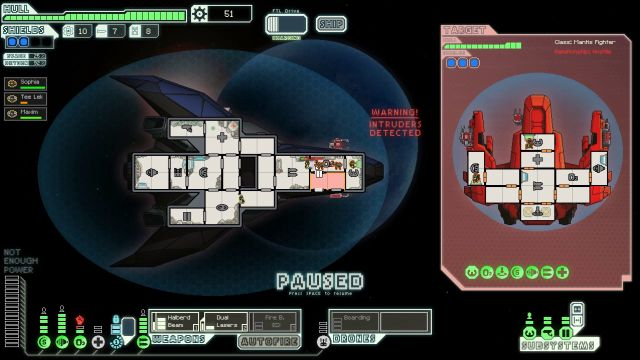
\includegraphics[width=\textwidth,height=\textheight,keepaspectratio]{./img/ftl.jpg}
	\caption{Captura de pantalla del videojuego FTL: Faster Than Light}
	\label{fig:ftl}
\end{figure}

\subsubsection{La creación de subgéneros}

Dado que perder todo el progreso y tener que empezar desde el principio sin haber conseguido nada más que la experiencia personal es algo que no atrae a mucha gente hoy en día (sobre todo porque la media de edad entre los jugadores está creciendo y cada vez es más gente que no puede pasar cietos de horas jugando), son numerosos los juegos que han añadido más elementos de progreso general para que el jugador no se sienta frustrado y consiga una recompensa de forma más inmediata. Estos elementos pueden ser nuevos personajes con los que jugar, puntos de experiencia generales o dinero con lo que poder equipar y mejorar desde un principio a nuestro personaje para poder llegar más lejos que la anterior vez, diferentes modos de juegos que se desbloquean al llegar a una cierta puntuación, etc.
También es común ver juegos que se basan en partidas cortas, de como mucho una hora, para que la repetición sea mayor y perder el personaje no sea un gran ``castigo'' que tener que afrontar, sino algo que forma parte del juego en sí.

Estos cambios en carácter que han sucedido durante los últimos años y que, de cierta manera, han modificado el género que \textit{Rogue} creó en un inicio, no siempre se han tomado positivamente por parte de la comunidad, que se suele quejar de que muchos títulos que se definen a sí mismos como \textit{roguelike} no contienen ciertas características (especialmente en tema de dificultad), que una vez definieron el género. Por este motivo se han definido subgéneros como el \textit{roguelite}, que toman muchas de esas ideas iniciales, pero añaden o ignoran otras muchas para crear un título que sea un poco más sencillo y no penalice tanto al jugador.

\subsection{Elementos \textit{roguelike} en nuestro proyecto}

En nuestro caso hemos creado un \textit{roguelike} similar a Rogue, no solamente estéticamente, pero también en diseño y funcionalidad. El usuario se moverá por un mapa aleatoriamente generado y luchará contra diferentes enemigos que intentarán eliminarlo de diferentes formas. En base al nivel que el usuario tenga, los enemigos serán más o menos complicados de batir y la recompensa por hacerlo será mayor.

El objectivo del juego es llegar lo más lejos posible dentro de la mazmorra. Cada vez que el jugador entra en un portal se añadirá un punto (el número de puntos se mostrará en la pantalla) y, cada vez que esto suceda, un nuevo mapa, con diferentes características y contenido, será generado, por lo que el jugador tendrá que intentar buscar este nuevo punto, batiendo enemigos y mejorando durante dicho recorrid. El juego es complicado, aleatorio y con una sensación de progreso, tal y como el género \textit{roguelike} especifica.

\begin{figure}[H]
		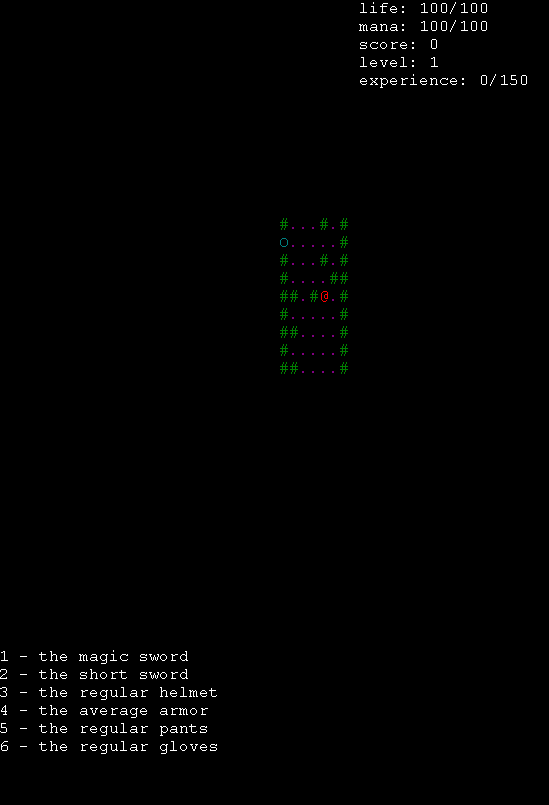
\includegraphics[width=140mm, height=185mm]{./img/roomsGameGeneral.png}
	\caption{Captura de pantalla de la interfaz de usuario de nuestro juego}
	\label{fig:roomsgamegeneral}
\end{figure}

\section{Problemas de la tecnología para ciertos sectores de la sociedad}
\label{sec:dificultadesfeedback}

Algunas de las razones que hacen de la tecnología un elemento prácticamente necesario hoy en día y que facilita su usabilidad crea, paradójicamente, una barrera para mucha gente que no puede disfrutar de ella, dificultado su día a día enormemente.

En esta sección hablaremos sobre algunos de los problemas que tantos invidentes como daltónicos se encuentran actualmente a la hora de usar diferentes programas (especialmente videojuegos) y cómo, en bastantes ocasiones, solventarlos no es requiere realizar nada más que prestar un poco de atención y tener ciertos simples aspectos en cuenta, lo que clarifica que muchas de estas limitaciones son dadas más por el desconocimiento que por la dificultad o coste de implementar una solución.

\subsection{Dificultades a las que se enfrentan los invidentes}

Las dificultades que tienen invidentes o personas con diferentes grados de ceguera en nuestra sociedad es enorme y, tristemente, los dispositivos tecnológicos y software no se ven excluidos de esta lista, a pesar de que han sido muchos los avances que hemos podido observar durante los últimos años.
No poder hacer uso de una interfaz gráfica o ver lo que está sucediendo en la pantalla es un problema que automáticamente imposibiliza el uso de la mayoría de las aplicaciones y videojuegos en su totalidad. Incluso navegar por internet, donde la mayoría del contenido es texto que puede ser leído fácilmente por un lector de pantalla, puede llegar a ser un quebradero de cabeza si cierta parte de ese contenido está en flash (el lector no podrá hacer nada en este caso), los enlaces a redes sociales están en posiciones poco recomendables (dado que su contenido se puede llegar a reproducir y generalmente son un suplicio saltarlos), algunos de los nombres usados en programas software son poco descriptivos y dificultan su correcta identificación, etc.

\subsection{Cómo solventar parte de estos problemas para los invidentes}

Uno de las primeros problemas que nos comentaron en la charla de la ONCE es que muchos de los desarrolladores que programan algo específicamente para ciegos no tienen en cuenta que, la mayoría de las veces, hay gente que puede ver a su alrededor que les puede describir lo que está sucediendo en la pantalla, por lo que es muy importante crear una interfaz que esté actualizada y muestre la misma información que la persona invidente reciba.
También es necesario dar la posibilidad al usuario de repetir el contenido generado, dado que algunos lectores tienen problemas para leer ciertos caracteres o lo que leen no es del todo claro y, por lo tanto, debe de ser fácilmente repetido.

Algunos videojuegos han visto versiones adaptadas para invidentes, la mayoría de ellas desarrolladas por la comunidad y no por las empresas iniciales, o nuevos títulos que se centran en ofrecer una experiencia revolucionaria desde el principio. Un buen ejemplo de ello es Shades of Doom\footnote{\url{http://www.gmagames.com/sod.html}}, que solamente usa sonido (principalmente ruidos repetitivos) y muy pocas frases para que el jugador sea capaz de descubrir lo que tiene que hacer, dónde está y describir todos los elementos que un usuario vidente recibe en una interfaz gráfica.

\subsection{Cómo hemos solventado el problema en nuestro proyecto}

En el proyecto, dado que se basa en la generación pseudo-aleatoria de frases, hemos creado descripciones para todos los elementos de la pantalla, por lo que el jugador siempre puede saber dónde se encuentra, qué hay a su alrededor, cuáles son sus características, etc. También hemos creado una ventana que se encuentra al lado del juego y donde se van guardando todas las frases generadas, siendo la primera frase la última generada y leyéndose automáticamente por el reproductor de pantalla que esté siendo usado en ese momento (en nuestro caso se trata de \textit{NVDA}). De esta forma, una persona con visión siempre puede leer dicha frase y el jugador repetirla las veces que quiera. Además de que el jugador también puede recordar lo sucedido anteriormente gracias a que los mensajes permanecen en la pantalla.

\begin{figure}[H]
		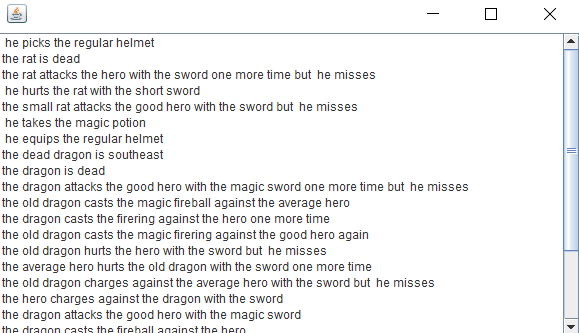
\includegraphics[width=\textwidth,height=\textheight,keepaspectratio]{./img/roomsGameTextArea.png}
	\caption{Captura de pantalla del area donde mostramos las frases generadas de nuestro juego para los invidentes}
	\label{fig:roomsgametextarea}
\end{figure}

\subsection{Dificultades a los que se enfrentan los daltónicos}

Daltonismo es un defecto genérico que afecta, aproximadamente, al 1\% de la población. Lo que en un principio parece como un pequeño inconveniente que no cambia mucho la vida de la persona que lo sufre, lo cierto es que hay muchas ocasiones en las que incluso ver un simple partido de fútbol americano correctamente puede convertirse en algo casi imposible para ellos \footnote{En \href{http://goo.gl/o3GkrP}{algunos partidos} los jugadores llevan camisetas con colores problemáticos.}. Incluso ver un mero mapa puede ser una complicación\footnote{\href{https://i.imgur.com/CMCywUU.jpg}{Resumen de algunos problemas que tienen los daltónicos a ver mapas}}.

En el mercado del ocio digital, donde los gráficos y paletas de colores juegan un gran papel en el arte del título, este problema se ve acentuado. La peor parte viene si parte de las mecánicas del juego necesitan que el jugador sea capaz de distinguir colores para obtener cierta información relevante; y esto es algo que sucede en numerosos títulos. En algunos casos es una pequeña molestia como en \textit{Borderlands}\footnote{Juego de acción en primera persona lanzado inicialmente en 2009 y que cuenta con varias secuelas} donde hay armas especiales que se diferencian, únicamente, por el color en el que se encuentra un determinado texto. Sin embargo, el mayor problema viene cuando estas limitaciones pueden llegar a arruinar el juego, como ocurre en \textit{The Witness}, un juego de puzzles mencionado en apartados anteriores en el que, para poder solventar muchos de dichos puzzles, requiere que el usuario distinga (o al menos tenga la información), distintos colores. 
También nos encontramos con juegos de lucha en dos dimensiones donde la única diferencia entre los escenarios del fondo y los personajes principales es el color de los mismos. No ver la diferencia complica a que el jugador detecte si un elemento está al frente o al fondo de dicho escenario.

\subsection{Cómo solventar parte de estos problemas para los daltónicos}
\label{sec:daltonicossolventar}

Para poder dar respuesta a esta cuestión, decidí preguntar en \textit{Reddit} a los usuarios daltónicos sobre cómo desarrollar un juego que sea adecuado para ellos \footnote{\url{https://goo.gl/d6cTqe}}. Fueron muchas las respuestas obtenidas, pero todo se puede resumir en un par de ideas.

La primera es que, en la medida de lo posible, nunca tengamos que diferenciar dos cosas distintas simplemente por el color. Tal y como un usuario comentó, si estamos desarrollando un juego naval y la diferencia entre un barco que está ``sano'' y uno que está ``roto'' es que cambiamos el color o la silueta del barco de verde a rojo, también podemos añadir chispas u otros elementos a mayores que faciliten la idea de que algo ha cambiado y ayude al usuario a apreciarlo visualmente con elementos a mayores. Del mismo modo, si tenemos un juego como \textit{Tetris} o \textit{Candy Crush} donde las piezas son relevantes, en vez de distinguirlas por color, podríamos hacerlas de diferentes formas o añadir una imagen a cada una de ellas.

La segunda idea es que, si es completamente necesario introducir diferentes colores para diferenciar ciertos elementos, o bien usamos colores que, generalmente, no crean ningún problema como el azul, amarillo, verde... (lo cual no nos garantiza que hayamos solventado el problema, dado que hay muchas formas de daltonismo y en algunas de ellas el usuario todavía puede tener problema diferenciándolos dependiendo del color contreto usado) o creamos una opción en el que podamos cambiar la paleta de colores usada. Hay algunos videojuegos (la mayor parte de ellos independientes), donde se da esta opción. 

\begin{figure}[H]
		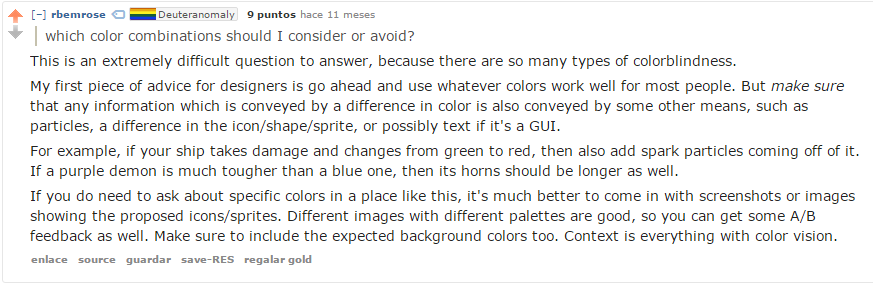
\includegraphics[width=\textwidth,height=\textheight,keepaspectratio]{./img/redditcolorblind1.png}
	\caption{Consejo para ayudar a los daltónicos a la hora de desarrollar un juego}
	\label{fig:roomsgamecolorblind1}
\end{figure}

\begin{figure}[H]
		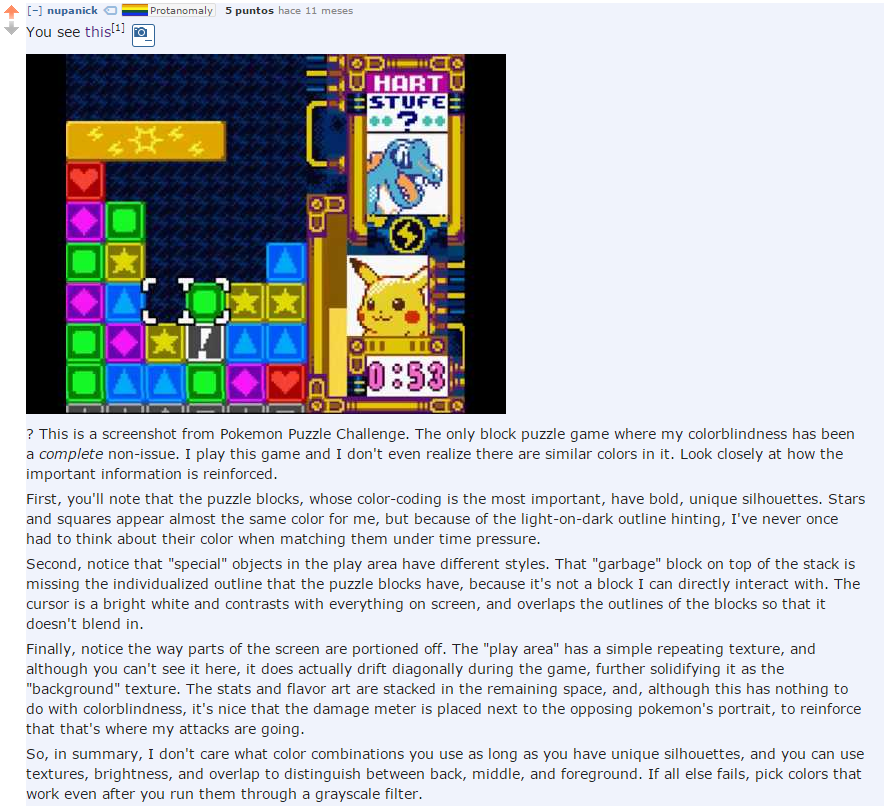
\includegraphics[width=\textwidth,height=\textheight,keepaspectratio]{./img/redditcolorblind2.png}
	\caption{Consejos y ejemplos para evitar que las personas daltónicas tengan problemas}
	\label{fig:roomsgamecolorblind2}
\end{figure}

\begin{figure}[H]
		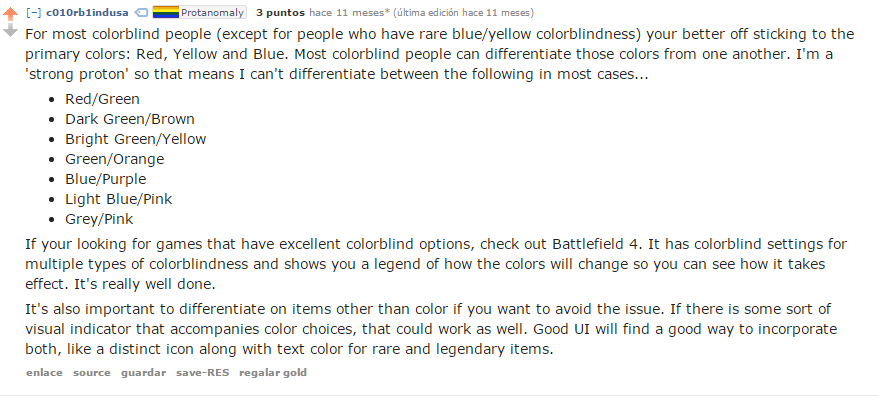
\includegraphics[width=\textwidth,height=\textheight,keepaspectratio]{./img/redditcolorblind3.png}
	\caption{Un usuario nos comenta la combinación de colores que son problemáticas}
	\label{fig:roomsgamecolorblind3}
\end{figure}

\subsection{Cómo hemos solventado el problema en nuestro proyecto}
\label{sec:solventadodaltonicos}

En nuestro caso, al haber preguntado de antemano a los usuarios, siempre tuvimos desde el primer momento la idea de crear la interfaz gráfica con soporte para daltónicos en mente, a pesar de que, al haber tenido en cuenta a las personas invidentes, cualquier persona podría jugarlo sin ninguna dificultad usando un lector de pantalla.

Todos los elementos que se encuentran en la interfaz gráfica están diferenciados con caracteres completamente diferentes por lo que, incluso aunque todos los colores fueran iguales, sería sencillo identificar cada elemento por su forma en vez de por su color. 

De todas maneras hemos creado una opción que cambia la paleta de colores a utilizar y facilita su visualización para aquellos usuarios que sufren de daltonismo.


        \chapter{Fundamentos Tecnológicos}

En este capítulo hablaremos sobre los fundamentos tecnológicos que vamos a usar en este proyecto y, si cabe, la razón por la que fueron elegidas. En primer lugar citaremos las herramientas que hemos usado y, en segundo lugar, las bibliotecas que hemos decidido utilizar en el programa en sí.

\section{Herramientas empleadas}

\paragraph{Java} Lenguaje de programación orientado a objetos cuya primera aparición fue en 1995. Es uno de los lenguajes de programación más utilizados en la industria y una de sus principales características es que es multiplataforma, es decir, puede ser ejecutado en cualquier sistema operativo que tenga la \textit{Java Virtual Machine} instalada sin necesidad de realizar cambios en el código (WORA\footnote{\textit{Write once, run anywhere}. Eslogan creado por Sun Microsystems para mostrar los beneficios de la multiplataforma}). Esta ventaja es esencial en nuestro caso, dado que la mayoría de las personas que pueden estar interesadas en el proyecto usan una gran variedad de sistemas operativos.

 \paragraph{Eclipse} Es un IDE\footnote{\textit{Integrated Development Environment}. Entorno de desarrollo integrado} usado para escribir código en múltiples idiomas. También incluye una serie de \textit{plugins} que facilitan y automatizan muchas de las labores a realizar como el uso de sistema de controles, ejecución de código y tests, herramientas de debug, autocompletado de código, etc.

 \paragraph{Git} Sistema de control de versiones distribuido introducido en 2005 y desarrollado principalmente por Linus Torvalds. Es el control de versiones referencia en la mayoría de empresas y proyectos de software libre gracias a su rapidez y, al ser distribuida, permite trabajar y realizar \textit{commits} del código sin necesidad de conexión a internet.

 \paragraph{GitHub} Plataforma de desarrollo colaborativo usada para alojar proyectos usando el sistema de control de versiones Git. La mayoría de proyectos de código abierto lo usan, dado que es gratuito, aunque también tiene la opción de almacenar el código de forma privada tras, previamente, realizar un pago.

 \paragraph{Listas de Correo} Las listas de correo son un método de comunicación muy usado por diferentes comunidades, especialmente en el desarrollo de software, que ayudan a los usuarios que participan en ellas a enviar correos a múltiples personas que lo deseen de forma anónima y, al mismo tiempo, tener un historial de las respuestas dadas por los mismos. En nuestro caso la hemos usado para comunicarnos con un grupo de usuarios y desarrolladores de videojuegos para invidentes.

 \paragraph{Reddit} Web creada en 2005 y que actualmente se encuentra en el top 50 de las más visitadas del mundo. Cuenta con una comunidad gigante que está dividida en muchísimos subgrupos dependiendo del tema a tratar. La hemos usado como una herramienta de feedback. Especialmente los \textit{subreddits} de daltónicos\url{https://www.reddit.com/r/ColorBlind/} y gente ciega\url{https://www.reddit.com/r/blind/}. 

\paragraph{Dia} Aplicación informática que permite la creación de todo tipo de diagramas. En nuestro caso lo hemos usado para crear los diagramas UML que se encuentran en esta memoria.

\paragraph{Gantt Project} Programa de software libre diseñado para la creación de diagramas de Gantt.

\paragraph{JSON} JavaScript Object Notation. Es un formato muy usado en APIs para intercambio de datos, similar a XML. En nuestro caso lo usamos para definir las gramáticas y diccionarios de nuestro proyecto, dado que es muy sencillo de leer y especificar. Hay numerosas bibliotecas que nos permiten analizar y trabajar con este formato en Java. La que nosotros usamos es \textit{Gson}.

\paragraph{\LaTeX} Sistema de composición de textos altamente usado por la mayoría de textos científicos dada la facilidad de su composición, simpleza, alta calidad y herramientas que a ayudan a la creación de fórmulas, inserción de imágenes y muchos otros elementos. Muy modificable. Es el sistema que hemos usado para la creación de este documento.

\paragraph{NVDA} Lector de pantalla de código libre para Windows. Orca es, en cierta medida, su equivalente en Linux.

\section{Bibliotecas empregadas}

\paragraph{Gson} Biblioteca usada para transformar archivos JSON a objetos de Java y viceversa.

\paragraph{JCurses} JCurses\footnote{\textit{The Java Curses Library}} es una biblioteca para el desarrollo de aplicaciones de terminal para JAVA. Es similar a AWT\footnote{\textit{Abstract Window Toolkit.} Kit de herramientas de interfaz de usuario de la plataforma original de Java}, pero basada en el sistema de ventanas Curses de UNIX.

\paragraph{Libjcsi} Biblioteca de representación gráfica que trabaja sobre JCurses y simplifica la tarea de representar y refrescar elementos del terminal.

        \chapter{Metodología}

En este apartado describiremos la metodología llevada a cabo en el proyecto. Una metodología es un conjunto de procesos, métodos y prácticas llevadas a cabo para asegurar, en la mayor medida posible, calidad en el producto final y en el tiempo acordado.

En nuestro caso, al ser un proyecto realizado por una sola persona y con un tiempo diario limitado, hemos optado por adaptar una serie de ideas y valores principales de varias metodologías.

\section{Desarrollo en cascada}

El desarrollo en cascada, también denominado como modelo en cascada, es una metodología con varias etapas donde, para pasar a la siguiente, es completamente necesario que la anterior haya acabado y esté completada.

Las ventajas que ofrece en desarrollo en cascada es que es muy sencillo de implementar en comparación con otras metodologías, requiere menos tiempo y capital para hacerlo funcionar de manera óptima y es usado con bastante frecuencia.

La mayor desventaja es que detectar un error en una de las fases finales puede significar tener que replantear los pasos tomados en las anteriores, perdiendo parte del progreso realizado.

\subsection{Etapas del desarrollo en cascada}

\paragraph{Análisis de requisitos}: 

En esta fase se definen y determinan los requisitos que el software debe de cumplir entre el desarrollador y el cliente. Generalmente se generan documentos que formalizan dichas decisiones para no tener que cambiarlas en el futuro, dado que un cambio en los requisitos puede significar cambiar gran parte del proyecto, por lo que llegar a un consenso es necesario.

\paragraph{Diseño}: 

Una vez del análisis haya finalizado, es hora del diseño. La idea principal es descomponer lo detallado durante el análisis de requisitos con el cliente y crear diferentes diagramas y diseños que ayuden a los programadores a entender lo que debe de ser realizado y cómo debe de funcionar, incluyendo pseudocódigo o algoritmos a alto nivel en caso de que sea necesario.

\paragraph{Implementación}:

En esta fase es donde se escribe el código fuente en base a lo espeficicado anteriormente, intentando dar gran importancia a la reutilización del código siempre y cuando sea posible. También es importante tener en cuenta la creación de tests y la realización de las primeras pruebas preliminares por parte de los programadores.

\paragraph{Verificación}:

Este es el momento final en el que el cliente es capaz de probar lo desarrollado. El programa debe de estar bien testado por parte de los programadores para evitar la mayoría de los problemas que pueden ocasionarse en esta fase.

\paragraph{Mantenimiento}:

Una vez el software ha finalizado y se ha entregado al usuario final, empieza la fase de mantenimiento. En ella el usuario final pedirá que se resuelvan problemas, se añadan nuevas funcionalidades y se cambien otras ya añadidas en base a los nuevos requisitos que vayan apareciendo y no se tuvieron en cuenta en el principio. Esta es una de las fases más críticas, dado que se estima que alrededor de un 80\% de los recursos de un proyecto se emplean en el mantenimiento \footnote{\url{http://eu.wiley.com/WileyCDA/WileyTitle/productCd-0471170011.html}}.

\begin{figure}[H]
		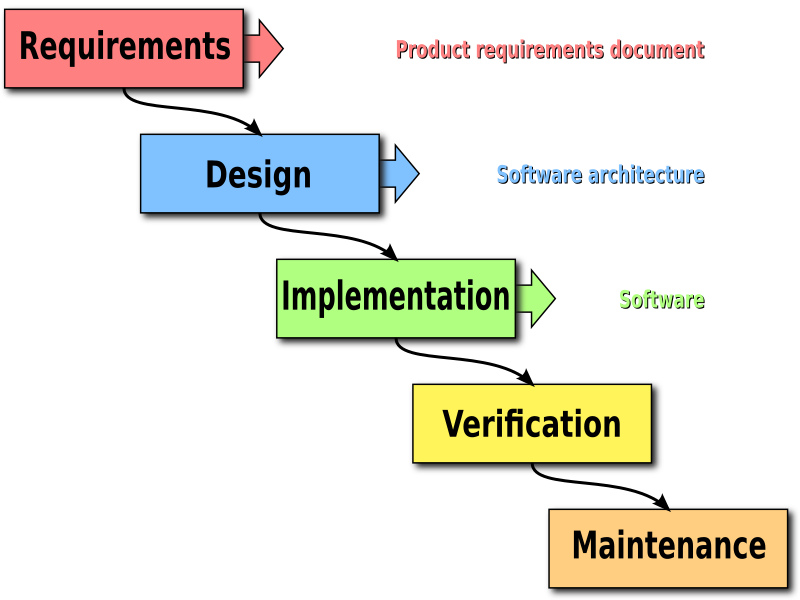
\includegraphics[width=\textwidth,height=\textheight,keepaspectratio]{./img/Waterfall_model.png}
	\caption{Estructura general de una etapa del desarrollo en cascada}
	\label{fig:cascadadesarrollo}
\end{figure}

\section{Scrum}

Scrum es una metodología ágil definida inicialmente por Hirotaka Takeuchi y Ikujiro Nonaka en 1986 \footnote{\url{https://cb.hbsp.harvard.edu/cbmp/product/86116-PDF-ENG}}. Su relativa sencillez, así como su flexibilidad y orientación al trabajo en equipo, hace que Scrum sea una de las metologías más usadas en el desarrollo de software, sobre todo en entornos laborales donde el equipo de desarrollo no es gigante (aunque su implementación también es posible en estos casos).

\subsection{Prácticas recomendadas y bases de Scrum}

Uno de los aspectos esenciales de scrum es el ``sprint'', que se trata de un bloque temporal de tiempo (generalmente de entre 2 y 4 semanas) donde el equipo de desarrollo trabajará para llegar a un objetivo determinado, generalmente acabar todas las tareas definidas para ese sprint. 
Al principio de cada sprint  el ``product owner'' y ``scrum master'' definirán las tareas que se querrán realizar en dicho sprint y que se encuentran en el backlog\footnote{Lista de tareas que se quieren realizar en el producto y que suele ir creciendo a medida que los usuarios encuentran fallos o necesitan nuevas funcionalidades. Generalmente el product owner es el encargado de organizar y decidir las tareas que tienen más prioridad}. Todos los integrantes del grupo de desarrollo, así como el propio product owner y scrum master, decidirán cuánto esfuerzo o tiempo llevará realizar cada tarea (hay algunas formas de decidir esto, como planning poker, pero no es muy relevante en nuestro caso), dividiéndola en tareas menores en caso de que sea demasiado grande. También se decidirá quién hará qué.

Durante cada día del desarrollo hay una pequeña reunión llamada ``sprint stand-up'' donde cada desarrollador comenta brevemente lo que ha hecho el día anterior, qué tiene planteado realizar ese día y si se ha encontrado con algún problema que le impida continuar.

Al acabar cada sprint, el equipo se reúne de nuevo para analizar lo que ha ido bien, qué problemas hubo y las mejoras que se tener en cuenta de cara al futuro. De esta manera, cada nuevo sprint será más preciso (dado que sabremos la cantidad de trabajo que cada desarrollador es capaz de hacer en el periodo definido de tiempo) e incluirán el ``feedback'' de los propios programadores.

Estas son las características eseciales de Scrum, pero al tratarse de una metodología ágil, nada es inamovible. Dependiendo del equipo y de las necesidades del mismo, se pueden cambiar o introducir nuevas ideas que mejoren el proceso para ese grupo de programadores en concreto.

\begin{figure}[H]
		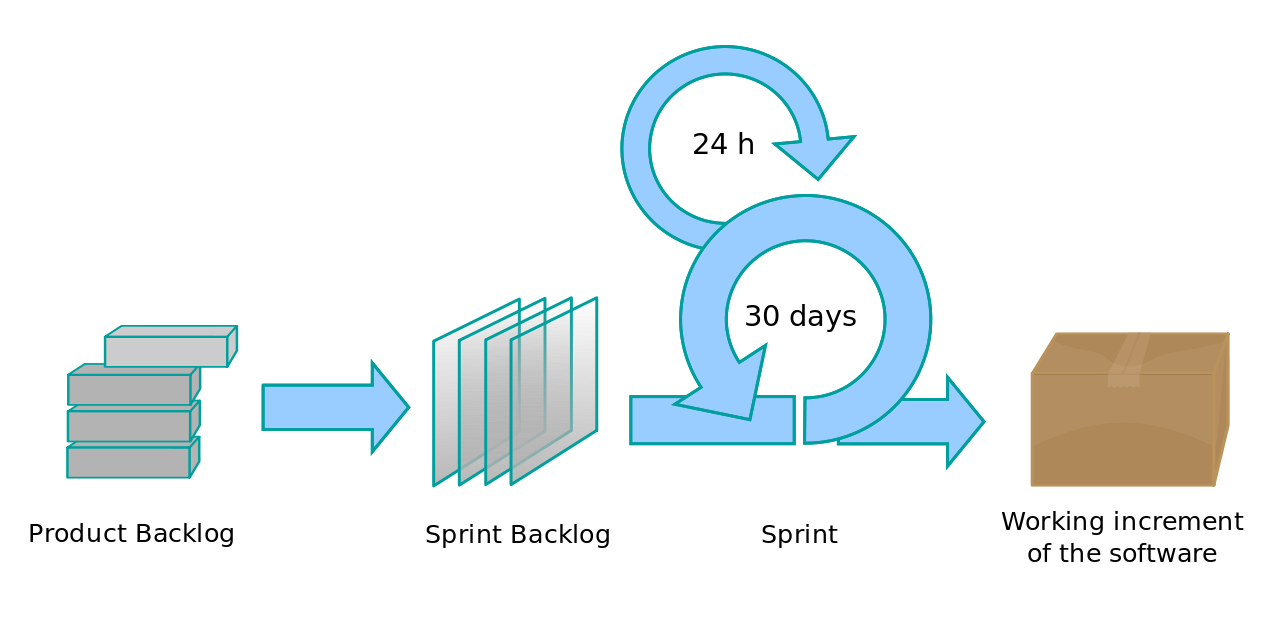
\includegraphics[width=\textwidth,height=\textheight,keepaspectratio]{./img/scrumprocess.png}
	\caption{Proceso concreto de scrum. En este caso el sprint dura 4 semanas}
	\label{fig:scrumproceso}
\end{figure}

\subsection{Valores de Scrum}

\subsubsection{Concentración}

Al tener que finalizar las tareas asignadas al final del sprint, la concentración del equipo en general y de cada uno de los miembros es esencial. Para logar este objetivo, el product owner es el encargado de responder las preguntas del resto de la compañía en nombre de los desarrolladores y solamente molestarlos en caso de que sea realmente necesario. 

\subsubsection{Coraje}

Dado que Scrum es una metodología de equipo, la ayuda entre cada uno de los miembros es algo esencial. De la misma forma, cada persona debe de ser capaz de enfrentarse a nuevos retos y asumir nuevas responsabilidades para que, en conjunto, el producto final sea el deseado. 

\subsubsection{Compromiso}

Cada integrante tiene que saber lo que puede hacer y comprometerse a ello. Una vez la reunión inicial se haya completado, es importante que cada uno sepa lo que tiene que hacer y pregunte en caso de que no tenga algo claro o crea que no puede llegar a terminar lo especificado durante la reunión. Cada programador debe de comprometerse con lo establecido para lograr el éxito del equipo.

\subsubsection{Sinceridad}

Ser capaz de asumir los errores es la clave para mejorar y evolucionar como un equipo. Si un miembro del equipo de desarrollo se queda estancado en un problema y no avisa al resto de sus compañeros, el sprint en su totalidad puede llegar a fracasar. Asumir responsabilidades, errores y pedir ayuda cuando sea necesario debe de ser una práctica habitual en Scrum.

\subsubsection{Respeto}

Similar al anterior punto. Al trabajar en equipo es imprescindible que tanto los logros como los fracasos se tomen como una nueva forma de aprender y mejorar, por lo que el respeto mutuo y asumir los errores es la mejor forma de evolucionar, tanto individualmente como en equipo.

\section{Metodología elegida}
\label{sec:metodologiaelegida}

Mayoritariamente hemos usado una metodología en cascada con algunos elementos de Scrum.

Para las características grandes del proyecto como la creación de los mapas, enemigos, sistema creación de frases, etc. nos hemos basado en cascada para analizar lo que tenemos que realizar, crear el diseño, implementarlo (empezando siempre por los tests, tal y como comentaremos a continuación) y verificarlo. Sin embargo, y dado que los juegos tienden a querer mejorarse continuamente con nuevos elementos de diferente importancia y tamaño (tanto de nuestra parte como de la gente que lo ha probado), tiene sentido mantener un backlog con todas las nuevas ideas y \textit{feedback} recogido, algo de lo que Scrum es maestro. También hemos seguido la idea de la creación de tareas cortas (de no más de 8 horas, en caso de que haya algo de mayor cantidad deberá de ser dividido en subtareas) y sprints, donde cada mes intentaremos tener un elemento del juego finalizado con varias tareas finalizadas a final de cada semana. De esta manera somos capaces de seguir más fácilmente el progreso que hemos realizado y tenemos constancia de los nuevos elementos que queremos implementar en un futuro, así como los bugs que arreglar en próximos sprints.
Al acabar con el núcleo del juego, la mayor parte de las tareas a realizar a continuación son pequeños cambios y nuevos elementos que no trastocan el diseño realizado del proyecto, por lo que seguir una metodología ágil como scrum es el mejor paso a seguir para terminar las tareas más relevantes lo antes posible.

Por último, también hemos seguido la práctica de \textit{test driven development} (desarrollo guiado por pruebas) cuya base está en, por cada nueva tarea a realizar, implementar primero los tests unitarios (que, lógicamente, fallarán) y luego programar la solución en sí para que el test sea válido, refractorizando la solución en caso de que no sea la ideal. Esto nos dará desde el primer momento una clara idea de lo que queremos hacer antes de ponernos con la implementación y nos asegurará de que siempre tendremos el test hecho.
        \chapter{Planificación y Seguimiento}

        \chapter[Análisis de Requisitos]{Análisis de Requisitos globales}

En este capítulos explicaremos el proceso de análisis de requisitos llevados a cabo para la elaboración de la aplicación y toda la información recibida por la comunidad.

\section{Consultas con la comunidad}

\paragraph{Blabla} Blabla

\subsection{Resumen}
	\paragraph{Blabla} Blabla

\section{Análisis de otros elementos}
Otros proyectos de accesbilidad o juegos.

\section{Requisitos del aplicativo}
Con toda la información obtenida y pensada, creamos una lista con los casos de uso que nuestro proyecto debe de cumplir.

\begin{itemize}
  \item \textbf{Whatever} Blabla
\end{itemize}

FIGURA DE CASOS DE USO UML. Hacer referencia.

% \begin{figure}[h!]
%     \centering
%     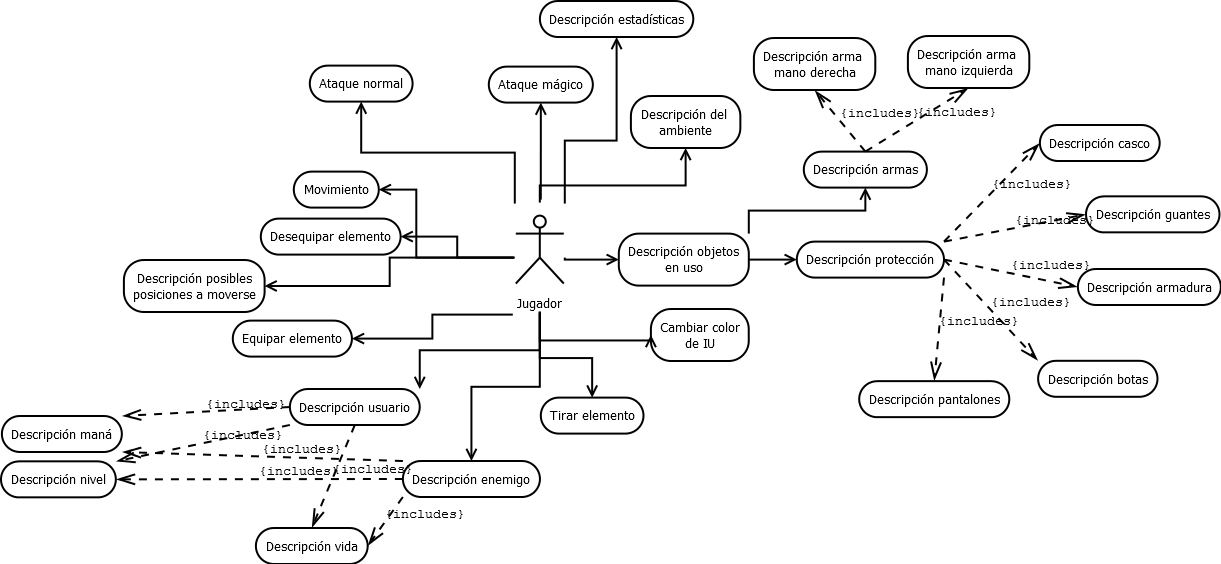
\includegraphics[width=0.9\textheight,angle=90]{img/casosdeuso.png}
%     \caption{Diagrama UML de casos de uso de la aplicación}
%     \label{fig:casosdeuso}
% \end{figure}

        \chapter{Diseño e Implementación}

En este capítulo mostraremos los detalles del diseño e implementación de diferentes partes del juego, aplicando principios de Generación Automática de Lenguaje Natural \cite{Reiter_and_Dale_2000b} y otras técnicas de Procesamiento de Lenguaje Natural,\cite{JurMar2009a}\cite{book:statisticalfoundations} así como buenas prácticas de programación\cite{Nystrom2014a}.

\section{Gramáticas y frases}

La parte correspondiente a la definición de gramáticas y generación automática de frases es la más relevante e innovadora del proyecto y la que lo diferencia del resto de juegos de similares características.

\begin{figure}
    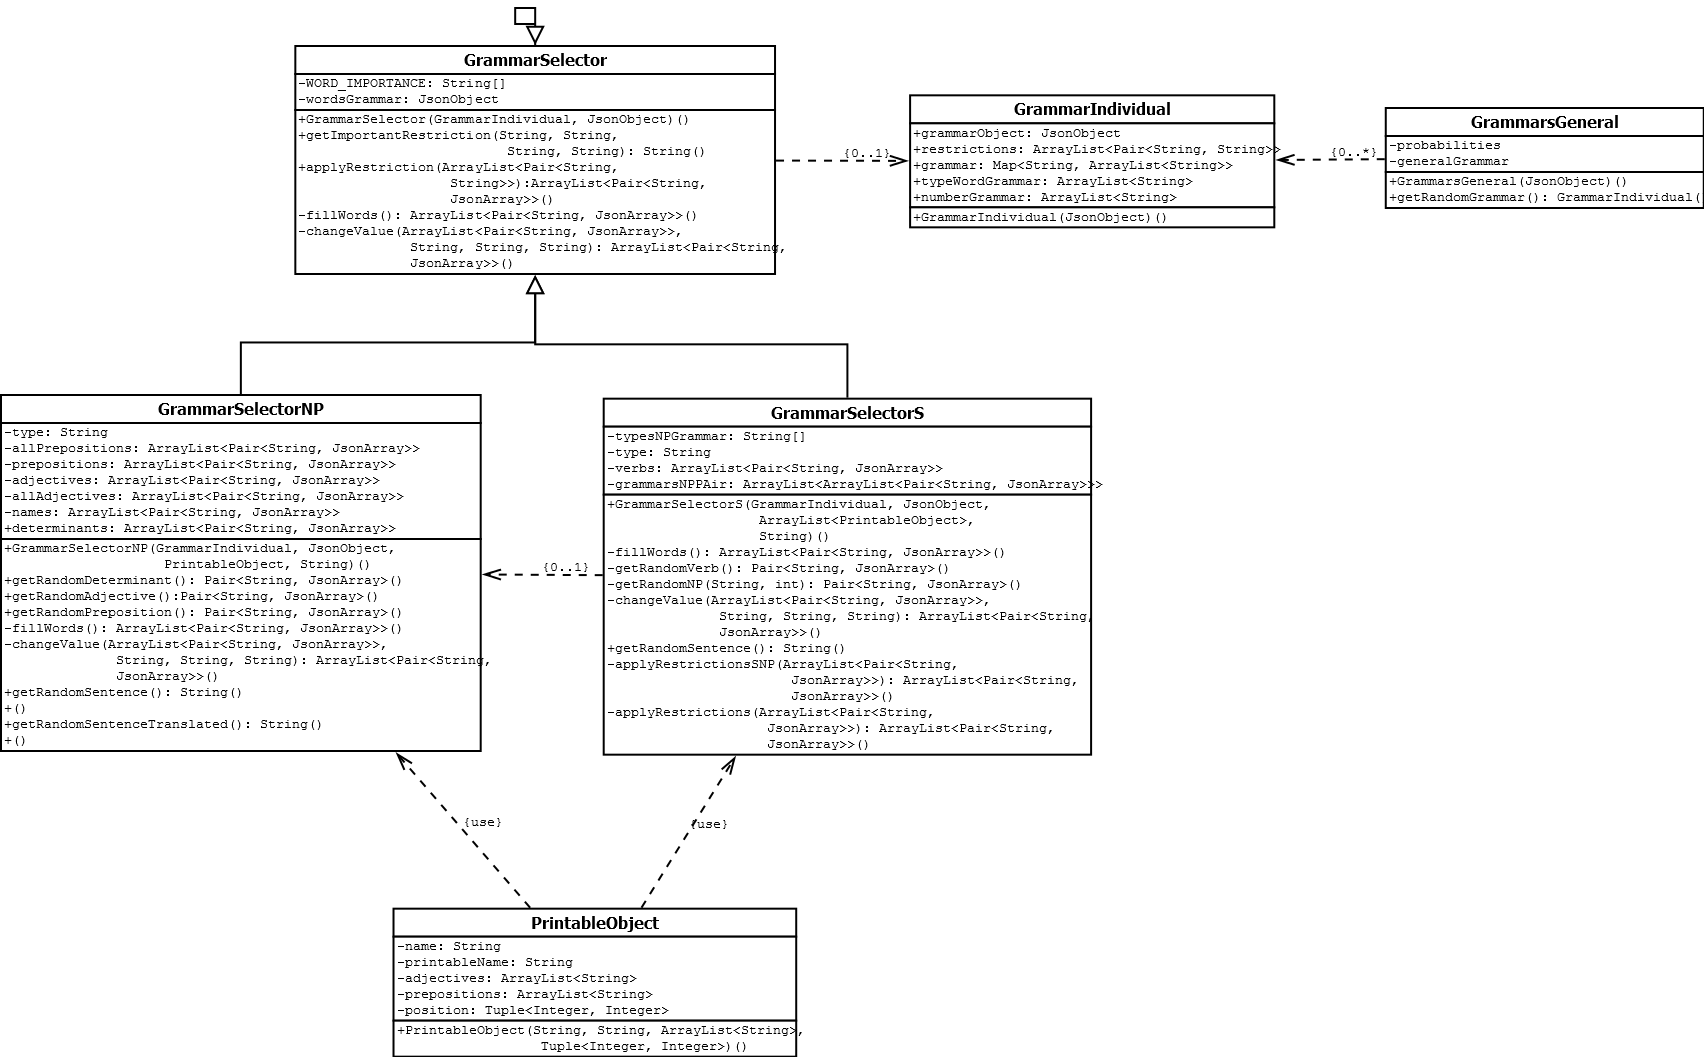
\includegraphics[width=1.5\textwidth,height=1.5\textheight,keepaspectratio,angle=90]{./img/grammarDiagram.png}
  \caption{Diagrama de clases de las gramáticas}
  \label{fig:clasesgramaticas}
\end{figure}

Tal y como se muestra en la Figura ~\ref{fig:clasesgramaticas}, la parte esencial de este módulo consta de seis clases, cuyo funcionamiento detallamos a continuación.

\subsection{Explicación general del funcionamiento}

Tenemos dos clases (\texttt{GrammarSelectorS} y \texttt{GrammarSelectorNP}) que se encargan de generar las frases en base al nombre o nombres sobre los que queremos obtener información. Esta frase se generará en base a gramáticas y diccionarios dados. La clase \texttt{GrammarSelectorNP} crea sintagmas nominales mientras que \texttt{GrammarSelectorS} crea frases usando, a su vez, dichos sintagmas nominales. Ambas usan diccionarios y gramáticas para el idioma concreto especificado en el archivo de configuración \textit{language.properties} (inglés en este caso que constituye el idioma por defecto):

\begin{verbatim}
language=EN
\end{verbatim}

\noindent Parte de la dificultad de generar estas frases está en que los elementos de la misma deben ser congruentes entre sí en base a las restricciones del idioma en cuestión. Por ejemplo, en el caso del español, los nombres, adjetivos y determinantes de una frase nominal deben coincidir en género y número, mientras que en inglés el género no es tenido en cuenta y, en el caso de los adjetivos, tampoco el número. Este tipo de restricciones vienen dadas por las gramáticas, que están especificadas en archivos JSON y que se comentarán más adelante.

Una vez detectemos que dos de las palabras no coinciden, cambiaremos la flexión de la palabra en base al tipo de la incongruencia (número en el caso del inglés). Por ejemplo, un adjetivo o determinante respecto a un sustantivo.

\begin{lstlisting}[language=java]

if (toChange.equals(value1)) {
    changeToValue = JSONParsing.getElement(restrictions1, type + "opposite");
    typeChangeToValue = typeFirstRestriction; 
     
} else {
    changeToValue = JSONParsing.getElement(restrictions2, type + "opposite");
    typeChangeToValue = typeSecondRestriction;
}
this.changeValue(sentenceArray, toChange, changeToValue, typeChangeToValue);

\end{lstlisting}

\noindent De esta manera, siempre que haya una discordancia entre algunos de los constituyentes de una frase, iteraremos entre sus elementos buscando una solución que sea coherente, cambiando sucesivamente la flexión de las palabras de menos rango dentro de dicha frase para que se adapten al resto.

La clase \texttt{GeneralGrammar}, por su parte, obtiene la información de varias gramáticas, ya que es así como vienen dadas en el fichero, puesto que para describir una misma situación puede haber varias gramáticas aplicables válidas, lo que concuerda con el concepto de \emph{variedad lingüística} del lenguaje humano,\cite{AraWeiBomKos2000a} es decir, cómo nuestro lenguaje permite expresar una misma idea o mensaje de diferentes formas. Por ejemplo, ``el héroe ataca al dragón'' y ``él se lanza contra el dragón con la espada mágica''. 
Para ello la clase \texttt{GeneralGrammar}, dispone de una función que devuelve una gramática individual (de la clase \texttt{GrammarIndividual}) de entre todas las disponibles para una situación determinada y es la que usaremos a la hora de generar la frase en sí. Es decir, cuando queremos generar una frase para describir una situación en concreto (por ejemplo cuando un personaje ataca a otro), seleccionaremos una de las gramáticas de entre todas las que estén disponibles para este tipo de encuentros en el idioma actual (esto lo realiza la clase \texttt{GrammarsGeneral}) y luego usamos esa gramática en particular (clase \texttt{GrammarIndividual}) para generar la descripción a mostrar al jugador. De esta forma no siempre usaremos la misma gramática para describir un mismo evento (o similar), aumentando la expresividad del sistema y evitando así resultar cargantes.

La clase \texttt{PrintableObject} es una superclase abstracta de la que heredan todos los objetos que pueden ser representados en el juego. Esta clase se encarga de obligar a que dichos objetos tengan ciertos atributos como el nombre o la capacidad de traducir su nombre a diferentes idiomas, así como una función que devuelve la posición en la que se encuentra respecto al usuario y que emplearemos a la hora de describir lo que hay alrededor del personaje.

\subsection{\textit{Input} de gramáticas y diccionario}

Tanto las gramáticas como los diccionarios empleados por el sistema son almacenados como ficheros JSON que el usuario puede modificar o intercambiar, lo que afectará al resultado de las frases generadas.

El sistema requiere tres archivos de entrada para un idioma dado, dos correspondientes a las gramáticas y el tercero correspondiente al diccionario. En el caso de las gramáticas, uno es empleado para generar los sintagmas nominales, mientras que con el otro generamos expresiones más complejas, en su mayor parte a partir de estos sintagmas nominales.

\subsubsection{Gramáticas: Sintagmas nominales}

A continuación mostramos un ejemplo de gramática generadora de sintagma nominal en inglés correspondiente a una estructura DETERMINANTE + ADJETIVO + NOMBRE:

\begin{lstlisting}[style=json]
"DETADJN": {
    "GM_1": {
        "S": 
            [
            {"DET_1": ""}, 
            {"ADJ_1": ""}, 
            {"N_1": ""}
        ],
        "restrictions": [
            {"DET_1.num": "N_1.num"},
            {"N_1.num": "ADJ_1.num"}
        ]
    }
}
\end{lstlisting}

\noindent En estas gramáticas especificamos, primero, el nombre del grupo de gramáticas (en este caso, \texttt{DETADJN}). Este identificador es usado por el programa y ayudará al traductor del sistema a entender el tipo que son.

El siguiente identificador es el nombre de esa gramática individual en particular. Éste no es empleado en el programa, pero su uso es necesario para poder definir varias de ellas sobre el mismo árbol. Por ejemplo, si queremos más gramáticas de tipo \texttt{DETADJN}, necesitaremos que se especifique un nombre distinto para cada una de ellas.

A continuación viene la definición de la gramática en sí. Primero nos encontramos con el apartado \texttt{S}, que es donde se almacenará su definición; y luego el apartado \texttt{restrictions} que, como su nombre indica, es donde especificaremos las restricciones morfosintácticas aplicables al anterior.

En el caso de nuestro ejemplo, en la parte de la gramática tenemos, en este caso, \texttt{DET\_1}, que es el primer determinante (y único) de la gramática; \texttt{ADJ\_1}, el primer y único adjetivo que tiene dicha gramática y \texttt{N\_1}, que es el nombre o sustantivo.
En las restricciones detallamos las partes que tienen que coincidir. En este caso solamente tenemos que el determinante, nombre y adjetivo tienen que ser iguales (congruentes) en número. Es decir, que ``the red swords'' no sería generada, sino que generaría ``the red sword''.

Este primer ejemplo era para inglés, cuyas restricciones son más sencillas que en otros idiomas como el español o el gallego, donde los nombres, determinantes y adjetivos no solamente tienen que coincidir en número, sino también en género. De este modo, la gramática equivalente para el español (y también gallego en este caso) sería la siguiente:

\begin{lstlisting}[style=json]
"DETADJN": {
    "GM_1": {
        "S": 
            [
            {"DET_1": ""},
            {"N_1": ""},
            {"ADJ_1": ""}
        ],
        "restrictions": [
            {"DET_1.num": "N_1.num"},
            {"N_1.num": "ADJ_1.num"},
            {"DET_1.gen": "N_1.gen"},
            {"N_1.gen": "ADJ_1.gen"}
        ]
    }
}
\end{lstlisting}

\noindent Nótese que no solamente hemos añadido el género a las restricciones (para que no podamos generar frases como ``la espada rojo'' o ``el espada roja''), sino que también hemos cambiado el orden del nombre y del adjetivo para que correspondan a la estructura típica en español. 

A la hora de cambiar la flexión de las palabras que componen la frase dispondremos de un array donde ordenar las palabras por \textit{rango} de relevancia. Un sustantivo es más importante, o tiene mayor rango que un determinante en cuanto a que el sustantivo, como núcleo de la frase nominal, es el que determina el género y número del sintagma con el que deben coincidir determinantes y adjetivos. Consecuentemente, si alguna de las restricciones no se cumple entre estos dos elementos, el determinante será el que cambiará para adaptarse al género y número del nombre, no al revés.

De esta manera podremos adaptar las gramáticas a diferentes idiomas de una forma sencilla y sin necesidad de modidifcar el código de la aplicación.

\subsubsection{Gramáticas: Estructuras complejas}

Las gramáticas para la generación de este tipo de estructuras también pueden hacer a su vez uso de aquellas gramáticas de sintagmas nominales. En este caso, a modo de ejemplo mostramos una gramática correspondiente a la descripción (sencilla) de un ataque: 

\begin{lstlisting}[style=json]
"ATTACK": {
	"S1": {
	    "S": [
	        {"DETADJN_1": ""},
	        {"V_1": ""},
	        {"DETADJN_2": ""},
	        {"SIMPLEPREP_1": ""}
	    ],
	    "restrictions": [
	        {"DETADJN_1.num": "V_1.num"}
	    ]
	},
	"S2": {
	    "S": [
	        {"GENERAL_1": ""},
	        {"V_1": ""},
	        {"SIMPLE_2": ""},
	        {"SIMPLEPREP_1": ""}
	    ],
	    "restrictions": [
	        {"GENERAL_1.num": "V_1.num"}
	    ]
	}
}
\end{lstlisting}

\noindent La estructura de esta gramática es la ya mencionada anteriormente. En este caso vemos que dentro de \texttt{ATTACK} disponemos de dos gramáticas distintas (éste es solamente un ejemplo, en el juego tenemos muchas más disponibles) y éstas llaman a sintagmas nominales como el anterior.
Con la primera gramática podríamos generar una frase del estilo ``The mighty dragon attacks the brave hero with the sword''. En este ejemplo cabe destacar que las restricciones se pueden definir no solamente entre palabras, pero también entre sintagmas nominales (siempre y cuando sea en comparación con una palabra que pueda ser cambiante, en este caso el verbo) y que los sintagmas nominales que son creados dentro de esta gramática tienen sus propias restricciones, por lo que siempre serán generadas de manera correcta.

\subsubsection{Diccionarios}

Al igual que las gramáticas, los diccionarios también están divididos por idiomas y son archivos JSON. Éste es un ejemplo de parte de un diccionario para inglés:

\begin{lstlisting}[style=json]
"DET": {
    "the": [
        {"num": ""},
        {"translation": "the"},
        {"numopposite": "the"},
        {"genopposite": ""}
        {"gender": ""}
    ]
},
\end{lstlisting}

\noindent El primer elemento, \texttt{DET}, especifica el tipo de palabra que es (determinante). El siguiente elemento especifica la palabra en sí (\texttt{the}). El resto de elementos estarán en un array de pares (CLAVE, VALOR), aunque en este caso no importa el orden de las mismas. La clave del primer elemento en esta lista es \texttt{num}, correspondiendo al número del término en cuestión, es decir, si el elemento es singular o plural (para esta palabra esta información es innecesaria, por eso es un string vacío) mientras que en \texttt{numopposite} guardaremos la flexión de la palabra en el número contrario (si la palabra es singular, entonces guardaremos la palabra en plural).
El segundo es \texttt{translation}. Todas las palabras entre los diccionarios serán las mismas o, por lo menos, las que están definidas en inglés también deben estarlo en otros idiomas. En este valor almacenaremos la traducción de esta palabra al idioma del diccionario que estaremos definiendo.
Los elementos \texttt{gender} y \texttt{genopposite}, al igual que con \texttt{num} y \texttt{numopposite}, almacenan el género de la palabra y la palabra de género contrario.

Retomando nuestro ejemplo anterior, con los determinantes en inglés no hay mucho cambio, pero en español sí que es bastante diferente:

\begin{lstlisting}[style=json]
"DET": {
        "el": [
            {"num": "sing"},
            {"translation": "el"},
            {"numopposite": "los"},
            {"genopposite": "la"},
            {"gen": "mas"}
        ],
        "la": [
            {"num": "sing"},
            {"translation": "la"},
            {"numopposite": "las"},
            {"genopposite": "the"},
            {"gen": "fem"}
        ],
        "los": [
            {"num": "plural"},
            {"translation": "los"},
            {"numopposite": "the"},
            {"genopposite": "las"},
            {"gen": "mas"}
        ],
        "las": [
            {"num": "plural"},
            {"translation": "las"},
            {"numopposite": "la"},
            {"genopposite": "los"},
            {"gen": "fem"}
        ]
    },
\end{lstlisting}

\noindent En este caso vemos que \texttt{numopposite} y \texttt{genopposite} apuntan ahora a \texttt{la} y \texttt{los}, que corresponden a la flexión en número y género, respectivamente. De esta forma  obtendremos el término que queramos siempre y cuando el programa precise obtener un tipo de palabra concreta en base a las restricciones que contenga la gramática.

\section{Otras partes del sistema}

Las gramáticas juegan un papel muy importante en el proyecto, pero hay otras partes relevantes del sistema que merecen una atención especial. Aquí mencionamos las más importantes:

\subsection{Interfaz de usuario para el texto generado}

Para que nuestro sistema pueda aprovecharse del software de lectura de pantalla empleado por usuarios invidentes, no basta simplemente con que saque el texto por pantalla. Debe hacerse de forma que el software de lectura pueda leerlo, lo que no es del todo trivial dado que hay que tener en cuenta diferentes aspectos para que el lector lea lo que queramos y no otras partes que no nos interesan. Más información sobre este tema se encuentra disponible en el Apéndice ~\ref{ref:instalacion} de esta memoria.

\subsubsection{Primer planteamiento: emplear \textit{pop-ups}}

La forma más sencilla de presentar este texto es mostrar un \emph{pop-up} cada vez que una frase es generada. De esta forma el usuario se enterará inmediatamente de lo que está sucediendo y, en caso de que haya una persona vidente a su lado, ésta también podrá leer la frase que se ha generado. Además, la frase no desaparecerá hasta que se presione la tecla de \textit{intro} o se haga click en \textit{Aceptar}, por lo que es muy sencillo reproducirla la cantidad de veces que se desee. La Figura ~\ref{fig:lastiterationui} muestra un ejemplo de uso sencillo para esta implementación.

\begin{figure}
    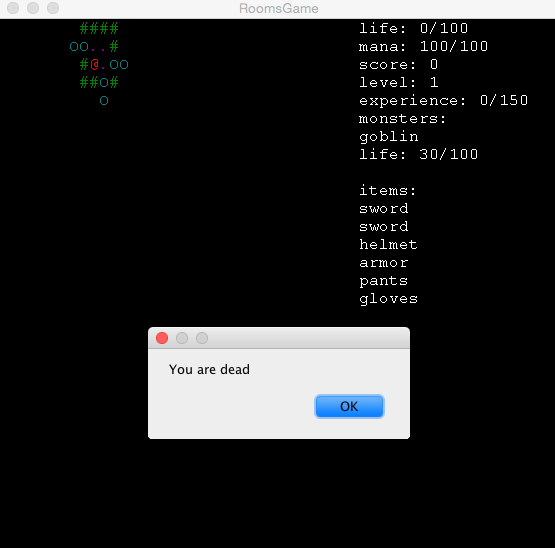
\includegraphics[width=\textwidth,height=\textheight,keepaspectratio]{./img/firstiterationui.png}
  \caption{Versión preliminar de la interfaz de usuario para el texto generado basada en el uso de \textit{pop-ups}}
  \label{fig:firstiterationui}
\end{figure}

\subsubsection{Segundo planteamiento: emplear una \textit{TextArea}}

En base al \textit{feedback} recibido de mano de los jugadores de prueba, decidimos abandonar esta prima solución por tres razones. La primera es que resulta desconcertante para el jugador vidente, dado que, en su caso, no es necesario. Esto se podría solventar añadiendo una opción que permita activar o desactivar esta función, aunque no es la mejor solución para este problema.
La segunda razón es que estos \textit{pop-ups} no son un mecanismo óptimo para mostrar salidas rutinarias, como en nuestro caso, pues rompe el ``flujo de trabajo''.
La tercera y última razón es que los usuarios invidentes no suelen hacer uso de elementos de este tipo, sino que están más acostumbrados a emplear áreas de texto donde se almacenan las últimas frases generadas por el programa en cuestión.

En base a estas ideas decidimos crear un área de texto que permanecerá abierta siempre y cuando el jugador no decida cerrarla, permitiendo a los usuarios videntes prescindir de ella. En el momento en que sucede algo en el juego que requiere generar una descripción, dicha descripción será enviada al área de texto, el ``foco'' de las aplicaciones cambiará para que se sitúe en esa ventana y el lector de pantalla leerá dicha descripción. Asimismo, generemos frases el ``foco'' seguirá en ese área de texto, si bien las teclas que pulsemos seguirán actuando sobre el juego para evitar romper el flujo de trabajo. El foco solamente volverá a la pantalla de juego cuando pulsemos una tecla que no genere una nueva frase.
De esta forma solucionamos todos los inconvenientes que los \textit{pop-ups} causaban a los usuarios, mejorando la interfaz gráfica y la accesibilidad del proyecto.

En la Figura ~\ref{fig:lastiterationui} se puede encontrar una captura de pantalla donde se muestra un ejemplo de uso para esta nueva implementación.

\begin{figure}
    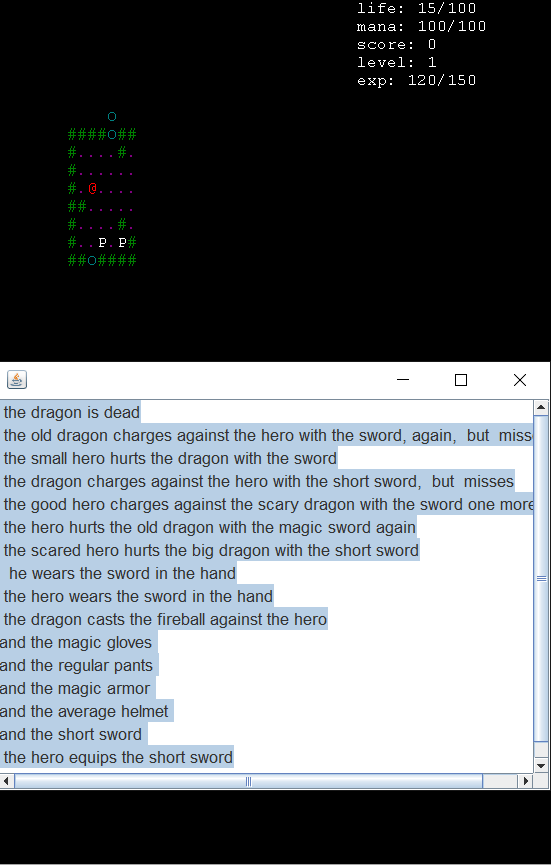
\includegraphics[width=\textwidth,height=\textheight,keepaspectratio]{./img/lastiterationui.png}
  \caption{Versión definitiva de la interfaz de usuario para el texto generado basada en el uso de una \textit{TextArea}}
  \label{fig:lastiterationui}
\end{figure}

\subsection{Generación aleatoria de mapas y elementos}

Como ya se indicó en la Sección ~\ref{game:roguelikeis}, la generación procedural aleatoria de los mapas y de los elementos que contienen \cite{Betts2014a} es una de las características de un juego de género \textit{roguelike}. A continuación explicaremos las decisiones tomadas a este respecto.

A la hora de generar el mapa en sí tenemos en cuenta tres elementos fundamentales: mapas (o mazmorras), habitaciones y puertas. Cada mapa generado consta de un conjunto de habitaciones, cuyo tamaño y forma cambia de manera aleatoria. Cada puerta une dos habitaciones por medio de un pasillo, asegurándonos que ninguna de las estancias queda sin la posibilidad de ser alcanzable por el jugador. También se han introducido columnas que se encuentran dentro de cada habitación para que tanto el jugador que controla el usuario como los enemigos tengan que esquivarlas y puedan usarlas en su favor en los combates entorpeciendo, además, el campo de visión de los personajes. Hay que tener en cuenta que ningún personaje puede moverse a una posición donde se encuentra una columna por lo que, a la hora de generarlas, se comprueba que no bloquean el acceso a la puerta o, si lo hacen, que haya otra entrada por la que se pueda acceder a dicha estancia.

\subsubsection{Primer planteamiento: Generación completamente aleatoria}

En un primer momento nuestra decisión fue la de generar todos los elementos de manera aleatoria, sin considerar ningún aspecto externo, pero manteniendo la generalidad en el código para poder cambiar su comportamiento en cualquier momento. Esto causaba que algunas mazmorras fueran muy complicadas cuando el jugador todavía no tenía el equipamiento necesario o nivel para enfrentarse a enemigos excesivamente poderosos o demasiado sencilla en otros momentos.

Este problema fue mencionado la primera vez que recibimos \textit{feedback} y por ello decidimos emplear una solución más elaborada.

\subsubsection{Segunda idea: Generador de encuentros}
\label{generadorencuentros}

En el mundo del rol, tener en cuenta ciertas características del personaje del jugador para generar elementos externos se denomina \textit{generación de encuentros}. De este modo, en vez de generar mapas, enemigos y elementos de manera completamente aleatoria, podemos generarlos en base al nivel que tienen ciertos personajes. Por ejemplo, si el personaje que controla el usuario tiene nivel 10, entonces los adversarios que se encuentren deberían ser de un nivel similar, entre 8 y 12, y así mantener un nivel de dificultad equilibrado, no demasiado fácil ni demasiado difícil, evitando que el jugador caiga en el tedio o en la frustración. De forma similar, los elementos que dichos oponentes suelten al morir, tales como espadas y armaduras, también deberían tener un poder proporcional para que la progresión tenga sentido y eliminar enemigos implique un cierto nivel de recompensa.

De esta forma, en base al nivel dado, podremos generar contrincantes con diferentes características que se adapten a lo que necesitamos. Mostramos un ejemplo de cómo generar un enemigo en una habitación en concreto:

\begin{lstlisting}[language=java]
Rat rat = new Rat(this.getMap(), this, position, new ArrayList<String>(), level);
\end{lstlisting}

\subsection{Comportamiento de los enemigos}
\label{sec:ia}

Como cabe suponer, los adversarios que nos encontramos en el juego se moverán de diferentes formas, por lo que tendremos que diseñarlo de una manera genérica que nos permita realizar esto de la forma más simple posible.
Para ello nos hemos basado en el patrón de diseño \textit{estrategia} porque se adapta perfectamente a nuestros requisitos.

Los tipos de movimiento que tenemos disponibles en el juego actualmente de cara a los enemigos son los siguientes:

\paragraph{RandomMovement:} Los enemigos son ``pasivos'', es decir, no atacarán a ningún personaje ni tampoco irán hacia él en ningún momento.

\paragraph{FollowingMovementDumb:} Los contrincantes que tengan este tipo de comportamiento son más ``agresivos''. Seguirán al jugador e intentarán atacarle, pero no se mueven de una forma óptima para lograr su meta, por lo que esquivarlos no suele ser muy complicado.

\paragraph{FollowingMovement:} Este tipo de comportamiento es el más complejo y ``agresivo''. El enemigo se moverá de manera precisa para llegar lo antes posible al usuario y usará todo tipo de tácticas para derrotarlo, tales como el uso de magia o atacándole cuerpo a cuerpo.

\noindent Gracias a nuestro diseño, crear nuevos tipos de comportamientos es una tarea trivial, ya que solamente tendríamos que implementar la interfaz \textit{Movement} con la única función que posee e insertar en él el código del nuevo tipo de movimiento.

La Figura ~\ref{fig:iaenemy} mostramos el diagrama de clases que hemos implementado en nuestro sistema y que contiene el patrón de diseño \textit{estrategia}, tal y como hemos comentado.

\begin{figure}
    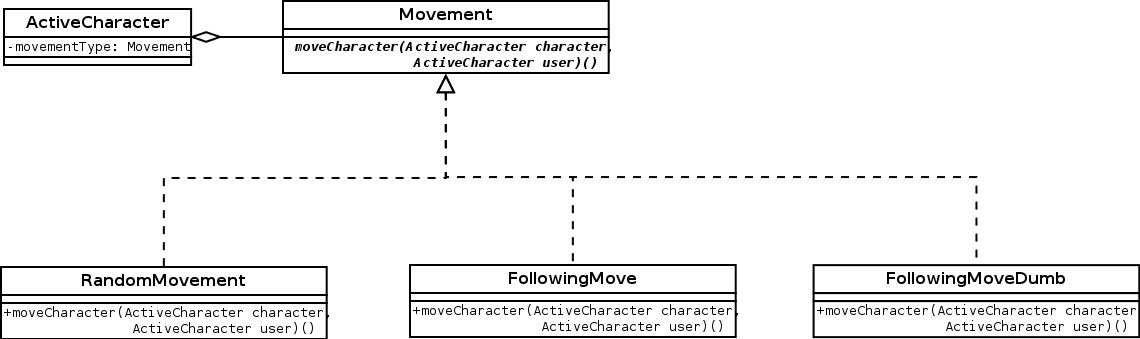
\includegraphics[width=\textwidth,height=\textheight,keepaspectratio]{./img/iaenemy.png}
  \caption{Diagrama de clases para el comportamiento de los enemigos}
  \label{fig:iaenemy}
\end{figure}

\subsection{Interacción entre objetos, personajes y hechizos}

La Figura ~\ref{fig:charactersitems} muestra las relaciones entre las clases abstractas e interfaces de los objetos, personajes, movimientos y hechizos de nuestro juego.

La clase \texttt{Character} contiene la información básica de los personajes, mientras que en \texttt{ActiveCharacter} se encuentra información adicional que posibilita que el personaje se mueva en base a una clase que implemente la interfaz \texttt{Movement} e interactúe con el resto de elementos del juego, por lo que es la clase de la que todos los enemigos heredan. Esto ayuda a que en un futuro puedan crearse personajes como vendedores que no necesiten moverse de manera sencilla. 
Todos los personajes pueden tener \texttt{Items}, que son consumibles (pociones) o elementos que el jugador puede equipar (espadas, cascos, botas, etc.). Sin embargo, éstos no tienen por qué pertenecer a ningún personaje, se pueden encontrar en el mapa para que el personaje que el jugador controla pueda cogerlos.
Por último, un personaje en concreto también puede tener diferente número de hechizos, representados en el diagrama por la clase abstracta \texttt{Spell}, que harán daño en cierta área y que también costarán maná. De la misma manera que con las clases \texttt{Movement} o \texttt{ActiveCharacter}, extenderla para crear nuevos hechizos es muy sencillo, lo que permite que los elementos primordiales del juego sean fácilmente extendibles.

\begin{figure}
    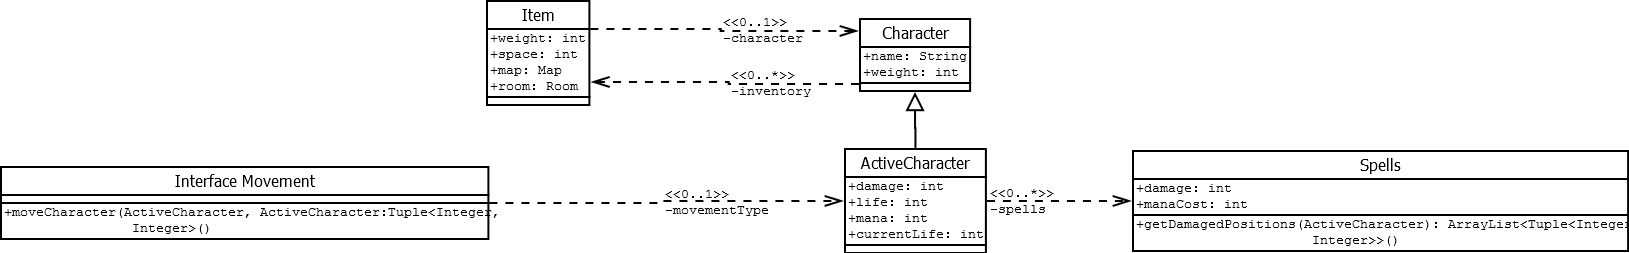
\includegraphics[width=\textwidth,height=0.15\textwidth]{./img/charactersitems.png}
	\caption{Diagrama de clases abstractas e interfaces sobre los objetos, personajes, hechizos y movimiento}
	\label{fig:charactersitems}
\end{figure}

\section{Herramientas empleadas}

En esta sección hablaremos sobre las tecnologías y herramientas empleadas en este proyecto y, si cabe, las razones por la que fueron elegidas. En primer lugar describiremos las herramientas y bibliotecas que hemos usado y, en segundo lugar, las herramientas de comunicación con usuarios y \textit{testers}.

\subsection{Herramientas software empleadas}

\paragraph{Java:} Este lenguaje de programación orientado a objetos es uno de los lenguajes de programación más utilizados en la industria. Una de sus principales características es que es multiplataforma, es decir, puede ser ejecutado en cualquier sistema operativo que tenga la \textit{Java Virtual Machine} instalada sin necesidad de realizar cambios en el código (WORA, \textit{``Write once, run anywhere''}). Esta característica es primordial en nuestro caso, dado que nuestros usuarios potenciales usan gran variedad de sistemas operativos, mayor incluso que respecto al usuario estándard	.

 \paragraph{Eclipse:}\footnote{\url{https://eclipse.org}} Es un IDE (entorno de desarrollo integrado) usado para escribir código en múltiples lenguajes. También incluye una serie de \textit{plugins} que facilitan y automatizan muchas de las labores a realizar, tales como el uso de sistema de controles, ejecución de código y tests, herramientas de \textit{debug}, autocompletado de código, etc.

 \paragraph{Git:}\footnote{\url{https://goo.gl/IKsKt5}} Sistema de control de versiones distribuido. Es el control de versiones referencia en la mayoría de empresas y proyectos de software libre gracias a su rapidez y, al ser distribuido, permite trabajar y realizar \textit{commits} del código sin necesidad de conexión a Internet.

 \paragraph{GitHub:}\footnote{\url{github.com}} Plataforma de desarrollo colaborativo usada para alojar proyectos usando el sistema de control de versiones Git. La mayoría de proyectos de código abierto lo usan, dado que es gratuito, aunque permite la opción de almacenar el código de forma privada previo pago.

\paragraph{JSON:} \textit{JavaScript Object Notation}. Es un formato muy usado en APIs para intercambio de datos, similar a XML. En nuestro caso lo usamos para definir las gramáticas y diccionarios de nuestro proyecto, dado que es muy sencillo de leer y especificar.

\paragraph{\textit{NVDA}:}\footnote{\url{www.nvaccess.org}} Lector de pantalla de código libre para Windows que lee el tipo de ventanas y texto que se encuentran en la pantalla, facilitando el uso del ordenador y otros dispositivos a los usuarios invidentes. 
Orca\footnote{\url{https://goo.gl/nW9UaZ}} es, en cierta medida, su equivalente en Linux. Otras alternativas son BrowseAloud\footnote{\url{https://goo.gl/GoghW7}} o Microsoft Narrator\footnote{\url{http://goo.gl/OAB7VC}}. Hemos elegido \textit{NVDA} por ser la alternativa libre más usada por este tipo de usuarios.

\paragraph{\textit{Gson}:}\footnote{\url{https://goo.gl/zPCXen}} Hay numerosas bibliotecas que nos permiten analizar y trabajar con este formato en Java. En nuestro caso hemos usado \href{https://goo.gl/zPCXen}{\textit{Gson}} para transformar archivos JSON a objetos de Java y viceversa.

\paragraph{JCurses:}\footnote{\url{https://github.com/sunhong/jcurses}} \textit{The Java Curses Library} es una biblioteca para el desarrollo de aplicaciones de terminal para JAVA. Es similar a AWT,\footnote{\textit{Abstract Window Toolkit.} Kit de herramientas de interfaz de usuario de la plataforma original de Java} pero basada en el sistema de ventanas \textit{Curses} de \textit{UNIX}.

\paragraph{Libjcsi:}\footnote{\url{www.slashie.net/libjcsi}} Biblioteca de representación gráfica que trabaja sobre JCurses y simplifica la tarea de representar y refrescar elementos del terminal.

\subsection{Herramientas de comunicación con usuarios y \textit{testers}}

\paragraph{Listas de Correo:} Las listas de correo son un método de comunicación muy usado por diferentes comunidades, especialmente en el desarrollo de software, que ayudan a los usuarios que participan en ellas a enviar correos a múltiples personas que lo deseen de forma anónima y, al mismo tiempo, tener un historial de las respuestas devueltas por los mismos. En nuestro caso las hemos usado para comunicarnos con un grupo de usuarios y desarrolladores de videojuegos para invidentes\footnote{\url{tiflo-juegos@googlegroups.com}} y recibir \textit{feedback} por parte de la comunidad.

 \paragraph{Reddit:}\footnote{\url{www.reddit.com}} Web creada en 2005 y que actualmente se encuentra en el top 50 de las más visitadas del mundo. Cuenta con una comunidad gigante que está dividida en muchísimos subgrupos dependiendo del tema a tratar. La hemos usado como una herramienta de \textit{feedback}. Especialmente los \textit{subreddits} de \href{https://www.reddit.com/r/ColorBlind/}{daltónicos}, de \href{https://www.reddit.com/r/blind/}{personas que sufren de ceguera}, \href{https://www.reddit.com/r/gamedev/}{desarrolladores de videojuegos} y \href{https://www.reddit.com/r/roguelikes/}{roguelikes}.

        \chapter{Conclusiones y trabajo futuro}

En este último capítulo detallaremos las conclusiones sacadas de la elaboración del proyecto y el posible desarrollo futuro del mismo.

\section{Conclusiones}

Realizar un proyecto de estas características no es sencillo. Dejando a un lado la parte técnica y de diseño, que nunca es trivial, en este caso se requiere un gran grado de investigación, análisis, asimilación del \textit{feedback} y determinación para poder sacarlo adelante. Sin embargo, también es cierto que durante su desarrollo siempre me he encontrado a una comunidad muy ilusionada por la existencia del proyecto y encantada de colaborar y resolver mis dudas.
Es una pena que algo tan esencial como son la mayoría de elementos tecnológicos de hoy en día (y su \textit{software} en particular) todavía no estén adaptados para que toda la parte de la población pueda usarlos sin grandes restricciones. Espero que con este proyecto haya gente que se anime a intentar hacer algo similar (o mejorar lo ya creado) y que entre todos podamos formar una sociedad donde no haya tanta discriminación tecnológica.

\section{Trabajo Futuro}

Cuando se crea cualquier tipo de \textit{software}, siempre existen mejoras y nuevas funcionalidades que puede ser añadidas para mejorar lo creado, sobre todo si se trata de un juego de \textit{software libre}, dado que las comunidades de desarrolladores y jugadores suelen ser bastante apasionadas. Ésta es la razón por la que, desde un principio, hemos establecido los elementos básicos a desarrollar para luego incluir otros elementos que no son tan esenciales.

Durante el desarrollo del proyecto se han tenido muchas ideas que hemos ido recopilando e implementando en caso de que las considerásemos necesarias. Actualmente todas estas ideas están recogidas en la página del proyecto en Github,\footnote{\url{https://github.com/dpenas/roomsgame/issues}} donde cualquier persona puede añadir su comentario o incluso realizar el cambio necesario y crear una \textit{pull request} para que sea incluido en el juego final.

De entre éstas, alguna de las ideas más interesantes con las que podemos mejorar el juego en el futuro son las siguientes: 

\paragraph{Creación de un menú de configuración:} En la actualidad no disponemos de un menú porque podemos realizar todo lo necesario dentro del propio juego. Sin embargo, y a medida que la cantidad de opciones de configuración crece, sería conveniente su creación para que nos mostrase lo que podemos cambiar sin tener que entrar en el juego en sí.

\paragraph{Añadir más variedad de enemigos y elementos:} La cantidad de enemigos diferentes que tenemos actualmente no es muy grande ya que desde el punto de vista académico aumentar dicha variedad no nos aportaba nada. Sin embargo, la experiencia de juego se beneficiaría teniendo más enemigos y objetos con los que interactuar, aunque sin olvidar que deben escalar de manera apropiada.

\paragraph{Integrar un modo historia:} El juego actual es abierto en el sentido de que las partidas son independientes entre sí y no hay un principio ni final definidos, sino que el usuario es el que crea, en cierta manera, su historia. 
No estaría de más integrar un nuevo modo de juego en el que se desarrolle una historia con argumento. Para ello se añadirían ciertos niveles y pantallas predefinidos mediante los cuales se hilvanaría la historia para aquellos usuarios que prefieran este tipo de aventuras.

\paragraph{Crear un tutorial:} Las instrucciones del juego se encuentran disponibles en la página de Github del proyecto, pero no estaría de más la creación de un tutorial o pantalla de inicio que explicase al usuario qué hacer y cómo desenvolverse por los entornos del juego.

\paragraph{Integrar un ``modo resumen'':} Con todas las frases que generamos durante la partida podríamos crear una especie de historia que relatase, en la medida de lo posible, lo que el jugador ha hecho durante dicha partida, dándole cierta importancia a los ``hitos'' conseguidos durante la misma. Otros \textit{roguelikes} como \textit{Dwarf Fortress} disponen de este elemento.\footnote{\url{http://www.bay12games.com/dwarves/}}

\paragraph{Incluir elementos sonoros:} Algunos juegos para invidentes solamente tienen elementos auditivos para informar al usuario sobre lo que tiene a su alrededor. En nuestro caso, al poder crear frases en base a unas gramáticas dadas, no resulta ser algo necesario, pero sí que podríamos crear una opción para que (en vez de) usar siempre descripciones, podamos reproducir sonidos a diferentes grados de volumen e incluso empleando técnicas de sonido tridimensional para informar al jugador sobre distintos elementos y enriquecer la atmósfera del juego. Por ejemplo, acompañar las descripciones de los combates con entrechocar de espadas.

\paragraph{Añadir más complejidad a las gramáticas:} Los textos generados se basan en las gramáticas que se hayan definido para el sistema, pero hay estructuras del lenguaje (como frases reflexivas), que son más complejas de crear que otras. Podríamos introducir estos nuevos elementos para que la cantidad de frases generadas y su variedad sea todavía mayor. 

\paragraph{Integrar recursos lógicos de terceros:} Tener un diccionario propio del sistema para el idioma en el que vayamos a jugar es necesario, dado que no todos los idiomas disponen del mismo tipo de recursos lingüísticos y su uso limitaría la cantidad de idiomas con los que podríamos jugar. Sin embargo, si el juego está, por ejemplo, en inglés, sí que podríamos usar recrsos como la base de datos léxica \textit{WordNet} para que, en vez de usar la palabra que se encuentra en nuestro diccionario, busque sinónimos en dichas bibliotecas, lo que aumentaría de manera significante la riqueza y expresividad del sistema. 

\paragraph{Añadir opción de jugar en base a una semilla:} Algunos \textit{roguelikes} o \textit{roguelites} como \textit{The Binding of Isaac: Rebirth},\footnote{\url{http://store.steampowered.com/app/250900}} permiten que el jugador introduzca un código que equivale a una semilla de aleatoriedad para que los elementos generados sean en base a esa semilla. Esto permitiría que los usuarios compartan partidas donde todo lo generado sea igual para ambos.

        \appendix
        \chapter{Escoger la licencia}

Cuando tenemos que escoger una licencia para un nuevo programa también debemos tener en cuenta las licencias de las bibliotecas y recursos que hemos usado en el mismo. Las bibliotecas que hemos usado en nuestro proyecto y sus respectivas licencias son éstas:

\begin{itemize}
  \item \textbf{Gson} Apache 2.0 license
  \item \textbf{JCurses} GNU Lesser General Public License v3
  \item \textbf{libjcsi} GNU Lesser General Public License v2.1
\end{itemize}

\noindent Como podemos apreciar, Gson usa una licencia Apache 2.0\cite{website:apachelicense} mientras que JCurses y libjcsi tienen GNU Lesser GPL \cite{website:gnulicense}.
La licencia de Apache 2.0 no es compatible con las versiones de GNU Lesser GPL anteriores a la 3, pero las versiones de GNU Lesser GPL son compatibles entre sí.
Por este motivo decidimos usar GNU General Public Licence v3, dado que es compatible con todas las licencias de las librerías que hemos usado.

        \chapter{Instalación e Instrucciones del Juego}
\label{ref:instalacion}

Nuestro \textit{roguelike} es software libre y el código fuente está libremente disponible en Github,\footnote{\url{https://github.com/dpenas/roomsgame}} al igual que varias versiones ejecutables del mismo. Dichas versiones ejecutables contienen un archivo \texttt{.jar} que solamente requiere tener una versión de JRE\footnote{\url{http://www.oracle.com/technetwork/java/javase/downloads/jre8-downloads-2133155.html}}{\footnote{Java Runtime Environment} superior a la 6 instalada en el sistema a usar. 

Para su ejecución basta con hacer doble clic en el archivo \texttt{.jar} o ir al directorio donde se encuentre dicho archivo e introducir:

\begin{lstlisting}[label=lst:bash,caption=Comando para la ejecución del videojuego]
java -jar game.jar
\end{lstlisting}

Para cambiar el idioma del juego accederemos al archivo \texttt{languages.properties} y cambiaremos el idioma a ES, GL, EN o NL para jugar en español, gallego, inglés u holandés, respectivamente. También es posible cambiar las teclas del propio juego. Las que vienen por defecto se puede encontrar en la wiki del proyecto.\footnote{\url{https://github.com/dpenas/roomsgame/wiki}}

En algunas ocasiones las frases generadas no se leen directamente. Esto viene causado por no tener activado el \textit{Java Access Bridge} o si no está instalada la versión correcta del mismo (se recomienda tener instalada la versión de 32 y 64 bits para evitar problemas). 
En sistemas Windows \textit{Java Access Bridge} se puede activar fácilmente de la forma siguiente:

\begin{itemize}
\item Ir a \textbf{Start \textrightarrow Control Panel \textrightarrow Ease of Access \textrightarrow Ease of Access Center}
\item Seleccionar \textbf{Use the computer without a display}
\item En la sección \textbf{Other programs installed}, seleccionar: \textbf{Enable Java Access Bridge}
\end{itemize}

\noindent Estas instrucciones deberían servir para Windows Vista y posteriores. En caso contrario, también se podrá hacer:

\begin{verbatim}
%JRE_HOME%\bin\jabswitch -enable
\end{verbatim}

donde \textit{\%JRE\_HOME\%} es el directorio donde Java está instalado.

\noindent Para otros sistemas operativos será necesario la descarga y activación de manera manual.\footnote{\url{http://www.oracle.com/technetwork/articles/javase/index-jsp-136191.html}}}



\end{document}

